%
% Szakdolgozatminta az Eszterházy Károly Katolikus Egyetem
% matematika illetve informatika szakos hallgatóinak.
%

\documentclass[
% opciók nélkül: egyoldalas nyomtatás, elektronikus verzió
% twoside,     % kétoldalas nyomtatás
% tocnopagenum,% oldalszámozás a tartalomjegyzék után kezdődik
]{thesis-ekf}
\usepackage[T1]{fontenc}
\PassOptionsToPackage{defaults=hu-min}{magyar.ldf}
\usepackage[magyar]{babel}
\usepackage{mathtools,amssymb,amsthm,pdfpages}
\usepackage{multirow, tabularx}
\usepackage{listings}
\usepackage{xcolor}
\usepackage{xurl, hyperref}
\usepackage{float}
\usepackage{enumitem}
\usepackage[justification=centering]{caption}
\footnotestyle{rule=fourth}

\newtheorem{tetel}{Tétel}[chapter]
\theoremstyle{definition}
\newtheorem{definicio}[tetel]{Definíció}
\theoremstyle{remark}
\newtheorem{megjegyzes}[tetel]{Megjegyzés}

\begin{document}

\institute{Matematikai és Informatikai Intézet}
\title{Gamifikált mobilalkalmazás fejlesztése az edzésmotiváció támogatására}
\author{Gunics Roland\\Programtervező Informatikus BSc}
\supervisor{Kovács Ádám\\Tanársegéd}
\city{Eger}
\date{2026}
\maketitle

\renewcommand{\lstlistingname}{kód}
\lstset{
    inputencoding=utf8/latin2,
    basicstyle=\footnotesize\ttfamily,
    columns=flexible,
    keepspaces,
    numbers=left,
    breaklines,
    postbreak=\hbox{$\mathcolor{red}{\hookrightarrow}$\ },
    xleftmargin=2cm,
    xrightmargin=2cm,
    frame=single,
    upquote,
    showstringspaces=false,
    literate=
        {á}{{\'a}}1 {Á}{{\'A}}1
        {é}{{\'e}}1 {É}{{\'E}}1
        {í}{{\'i}}1 {Í}{{\'I}}1
        {ó}{{\'o}}1 {Ó}{{\'O}}1
        {ö}{{\"o}}1 {Ö}{{\"O}}1
        {ő}{{\H o}}1 {Ő}{{\H O}}1
        {ú}{{\'u}}1 {Ú}{{\'U}}1
        {ü}{{\"u}}1 {Ü}{{\"U}}1
        {ű}{{\H u}}1 {Ű}{{\H U}}1
        {\$}{{\textdollar}}1
}
\lstdefinestyle{pseudostyle}{
    language={},
    backgroundcolor=\color{yellow!10},
    basicstyle=\footnotesize\ttfamily,
    breaklines=true,
    keywordstyle=\bfseries,
    commentstyle=\color{green!50!black}\itshape,
    stringstyle=\color{black},
    identifierstyle=\color{black},
}

\lstdefinestyle{pythonstyle}{
    language=Python,
    backgroundcolor=\color{yellow!10},
    basicstyle=\footnotesize\ttfamily,
    numbers=left,
    breaklines=true,
    frame=single,
    keywordstyle=\color{blue}\bfseries,
    commentstyle=\color{green!50!black}\itshape,
    stringstyle=\color{purple},
    identifierstyle=\color{black}
}

\lstdefinestyle{textstyle}{
    language={},
    basicstyle=\footnotesize\ttfamily,
    backgroundcolor=\color{gray!10},
    numbers=none,
    frame=single,
    breaklines=true
}

\lstdefinelanguage{TypeScript}{
    keywords={typeof, new, true, false, let, const, function, return, class, export, import, from, as, interface, type, extends, implements, public, private, protected},
    keywordstyle=\color{blue}\bfseries,
    ndkeywords={string, number, boolean, any, void, never, unknown},
    ndkeywordstyle=\color{blue},
    identifierstyle=\color{black},
    sensitive=true,
    comment=[l]{//},
    morecomment=[s]{/*}{*/},
    commentstyle=\color{teal}\itshape,
    stringstyle=\color{purple},
    morestring=[b]',
    morestring=[b]"
}

\lstdefinestyle{typescriptstyle}{
    language=TypeScript,
    backgroundcolor=\color{yellow!10},
    basicstyle=\footnotesize\ttfamily,
    numbers=left,
    breaklines=true,
    frame=single,
    keywordstyle=\color{blue}\bfseries,
    commentstyle=\color{green!50!black}\itshape,
    stringstyle=\color{purple},
    identifierstyle=\color{black}
}

\tableofcontents

\chapter*{Bevezetés}
\addcontentsline{toc}{chapter}{Bevezetés}

\begin{quote}
\centering
\label{quote_socrates}
    \emph{,,Bizony, kellemetlen dolog a hanyagság miatt úgy megöregedni, \\hogy még csak meg sem látta az ember, \\milyen lehetne a teste a legszebb és legerősebb állapotában.''\\ -- Szókratész~\cite{xenophon_memorabilia, nemeth1986}}
\end{quote}


A rendszeres testmozgás fenntartása sok ember számára jelenthet kihívást, különösen hosszú távon. Bár számos edzésalkalmazás érhető el, ezek többsége elsősorban funkcionális eszközként működik (edzéstervek, statisztikák, nyomon követés), és korlátozottan támogatja a felhasználói motiváció fenntartását. Ennek következtében a kezdeti lelkesedés gyakran csökken, és az edzési rutin megszakad. Ez különösen problémás ugyanis egy új viselkedés tartós szokássá válásához átlagosan mintegy 66 nap szükséges~\cite{lally2010habits}.

A szakdolgozat célja egy olyan edzőalkalmazás tervezése és megvalósítása, amely a hagyományos funkcionalitást gamifikációs és narratív elemekkel egészíti ki, ezáltal növelve a felhasználói elköteleződést és a hosszú távú motivációt.

A célfelhasználói csoport elsősorban olyan edzeni kívánó személyek, akik érdeklődnek a játékos megoldások iránt és nehézséget jelent számukra az edzés rendszeres fenntartása. A rendszer fő használati esetei közé tartozik az edzések rögzítése, a felhasználói fejlődés nyomon követése, különböző küldetések teljesítése, valamint egy interaktív, narratív alapú kalandélményben való részvétel.

A dolgozatban bemutatott megoldás egy teljes rendszer megvalósítása, amely magában foglalja a mobil frontend alkalmazást, a backend szolgáltatásokat, valamint a gamifikációs logikát. A rendszer kiegészül egy mesterséges intelligencia alapú komponenssel is, amely képes dinamikus, szöveges kalandok generálására, ezáltal személyre szabott élményt biztosítva a felhasználó számára.

A témaválasztást részben személyes motiváció is indokolta. A Szókratésznek tulajdonított idézet első alkalommal jelentős ösztönzést adott az edzés megkezdéséhez, azonban ez a motiváció hosszú távon nem bizonyult tartósnak. Ez a tapasztalat rávilágított arra a problémára, hogy a kezdeti lelkesedés fenntartása nehéz, amely közvetlen inspirációt jelentett a dolgozatban bemutatott rendszer megalkotásához.

A szakdolgozat forráskódja és az Androidra letölthető verzió az alábbi hivatkozásokon érhetők el:

\begin{itemize}
    \item GitHub (forráskód): \url{https://github.com/gunicsroland/D-D-Exercise}
    \item GitHub (build): \url{https://github.com/gunicsroland/D-D-Exercise/releases}
\end{itemize}

\chapter{Gamifikáció és motivációs háttér}

A modern mobilalkalmazások fejlesztése során egyre nagyobb hangsúlyt kap a felhasználói élmény (UX) és a hosszú távú felhasználói elköteleződés biztosítása. Különösen igaz ez az egészség- és fitneszalkalmazások esetében, ahol a rendszeres használat és a kitartás kulcsfontosságú tényezők. Több kutatás rámutat arra, hogy a pusztán funkcionális megközelítés gyakran nem elegendő a felhasználók motiválására, ezért kiegészítő motivációs eszközök alkalmazása szükséges~\cite{hamari2014does}.

A gamifikáció olyan módszertani megközelítés, amely játékmechanikák alkalmazását jelenti nem játék célú környezetben~\cite{deterding2011gamification}. Célja a felhasználói aktivitás növelése, az elköteleződés erősítése, valamint a kívánt viselkedésminták ösztönzése. A szakirodalom alapján a gamifikáció különösen hatékony lehet olyan területeken, ahol a felhasználók hosszú távú motivációja kritikus, például oktatásban, egészségügyben vagy életmódváltás során~\cite{hamari2014does}.

A motiváció szempontjából fontos különbséget tenni az intrinszik (belső) és extrinszik (külső) motiváció között~\cite{ryan2000intrinsic}. A jól megtervezett gamifikációs rendszerek képesek mindkét típus támogatására: rövid távon jutalmakkal ösztönöznek, hosszabb távon pedig a fejlődés és kompetencia érzését erősítik.

Azonban a gamifikáció alkalmazása nem minden esetben vezet pozitív eredményekhez. Nem megfelelő tervezés esetén a rendszer túlzottan a jutalmakra építhet, ami csökkentheti a belső motivációt, illetve hosszú távon érdektelenséghez vezethet~\cite{hanus2015assessing}. Emiatt kiemelten fontos a kiegyensúlyozott és felhasználó-központú tervezés.

A jelen szakdolgozatban bemutatott rendszer egy komplex gamifikációs megközelítést alkalmaz, amely ötvözi a klasszikus játékmechanikákat a modern technológiákkal, beleértve az adaptív rendszereket és mesterséges intelligencia alapú tartalomgenerálást is. Ez lehetővé teszi a személyre szabott élmények kialakítását, amely tovább növelheti a felhasználói elköteleződést és motivációt.

\section{Gamifikációs elemek}

A rendszer egyik fontos kiegészítő eleme a gamifikáció, amelynek célja a felhasználói élmény növelése, valamint az edzések véghezvitelének ösztönzése. 

A szakdolgozatban megvalósított rendszer a Dungeons \& Dragons (D\&D) nevű szerepjátékot veszi alapul, amely jól strukturált karakterfejlődési és jutalmazási mechanizmusokat biztosít. A D\&D inspiráció alapját a szintek, tapasztalati pontok (XP), valamint a karakterattribútumok képezik, amelyek alkalmasak a felhasználói aktivitás modellezésére.

\section{A Dungeons \& Dragons szerepjáték integrálása}

A gamifikációs rendszer központi eleme egy virtuális karakter, amely a felhasználót reprezentálja. A karakter különböző attribútumokkal rendelkezik, amik az aktivitásoknak és előrehaladásoknak megfelelően változnak.

A Dungeons \& Dragons által definiált hat alapvető tulajdonságra épül \cite[173.\ oldal]{dnd_player_handbook}, amelyek a karakter fizikai és mentális képességeit írják le:

\begin{itemize}
    \item \textbf{Erő (Strength):} a fizikai erő és teljesítőképesség mértéke.
    \item \textbf{Ügyesség (Dexterity):} a mozgáskoordinációt, gyorsaságot és reakcióképességet jelöli.
    \item \textbf{Állóképesség (Constitution):} a kitartást és fizikai ellenállóképességet reprezentálja.
    \item \textbf{Intelligencia (Intelligence):} a logikai gondolkodást, tanulási képességet és memóriát írja le.
    \item \textbf{Bölcsesség (Wisdom):} az észlelést, megértést és helyzetfelismerést jelenti.
    \item \textbf{Karizma (Charisma):} a személyiség hatását, kommunikációs és befolyásolási képességet méri.
\end{itemize}

Ezen felül az élmény mélyítéséért egyéb elemek lettek integrálva:

\begin{itemize}
    \item \textbf{Tapasztalati pontok (XP):} a felhasználó különböző edzések végrehajtásával tapasztalati pontokat szerez.
    \item \textbf{Szintek:} a megszerzett XP alapján a karakter szintet lép, amellyel az attribútumait tudja növelni.
    \item \textbf{Küldetések (questek):} az alkalmazás feladatokat kínál, amelyek teljesítése XP-vel és tárgyjutalmakkal jár.
    \item \textbf{Tárgyak:} a karakter tárgyai, amelyeket aktiválva ideiglenesen növelik az egyes attribútumokat.
    \item \textbf{Kalandok:} egy kiemelt elem, ahol az attribútumok szerepet kapnak egy LLM által generált D\&D történetben.
\end{itemize}


A D\&D alapú megközelítés egyik fő előnye, hogy jól strukturált fejlődési rendszert biztosít, amely hosszú távon is motiválhatja a felhasználót. A szintek elérése és a folyamatos fejlődés érzése hozzájárul a rendszeres használathoz~\cite{hamari2014does}.

A küldetések teljesítése rövid távú célokat biztosít, míg a szintek és attribútumok hosszabb távú fejlődést reprezentálnak. Ez a kettősség segít fenntartani a felhasználói elköteleződést.

\chapter{Technológiai áttekintés}
\label{chap_tech}

A mobilalkalmazás-fejlesztés napjainkban rendkívül sokféle megközelítéssel valósítható meg. A különböző platformok (iOS, Android) eltérő technológiai háttere miatt több fejlesztési irányzat alakult ki, amelyek különböző előnyökkel és hátrányokkal rendelkeznek. A megfelelő technológia kiválasztása nagymértékben függ a projekt követelményeitől, a fejlesztési időtől, valamint a célplatformoktól.  

A fejezet célja a projekt során alkalmazott fejlesztői eszközök, programozási nyelvek, keretrendszerek és infrastruktúra bemutatása. A választott technológiák meghatározása során fontos szempont volt a fejlesztési hatékonyság, valamint a széles körű közösségi támogatás. 

\section{Mobil fejlesztés}
A mobilalkalmazások fejlesztése három fő kategóriába sorolható: natív, webes és hibrid megoldások. Ezek elsősorban az alkalmazás felépítésében, a használt technológiákban és a platformfüggetlenség mértékében térnek el egymástól. A létező technológiákról egy összefoglaló látható \aref{tab_mobil_dev_comp}.\ táblázaton.

\subsection{Native (iOS -- Swift, Android -- Kotlin/Java)}
A natív alkalmazások kifejezetten egy adott operációs rendszerre készülnek, így magas teljesítményt és teljes körű hozzáférést biztosítanak az eszköz hardveres és szoftveres funkcióihoz. Azonban a különböző operációs rendszerek eltérő nyelveket használnak, ezért több kódbázist kell ebben az esetben fenntartani, ami növeli a fejlesztési költséget. iOS esetén ez jellemzően a Swift~\cite{iOS_languages}, míg Android esetén a Kotlin vagy Java. Játékok esetén, ahol igény van a magas teljesítményre előfordul a C++\cite{android_languages}.

\subsection{Webes alkalmazások}
A webes alkalmazások ezzel szemben böngészőben futnak, és nem igényelnek telepítést. Egyetlen kódbázisból működnek, általában HTML, CSS és JavaScript technológiákra épülnek, így platformfüggetlenek, azonban korlátozottabb hozzáféréssel rendelkeznek az eszköz natív funkcióihoz.

\subsubsection{Progresszív Web Alkalmazás}
A webes alkalmazások egyik speciális típusa a Progresszív Web App (PWA). A PWA-k szintén böngészőalapú programok, azonban lehetőséget biztosítanak arra, hogy a felhasználó azokat telepítse az eszközére. Ezen kívül offline működést, gyorsabb betöltést és a natív alkalmazásokhoz hasonló felhasználói élményt kínálnak, például teljes képernyős megjelenéssel és értesítések támogatásával~\cite{microsoft_PWA}.

\subsection{Hibrid alkalmazások}
A hibrid alkalmazások a natív és webes megközelítések ötvözetét jelentik: webes technológiákkal készülnek, de egy natív konténerben futnak, így telepíthetők alkalmazásboltokból, miközben részben hozzáférnek az eszköz funkcióihoz. Előnyük, hogy egyetlen kódbázisból több platform is kiszolgálható, ami csökkenti a fejlesztési időt és költségeket~\cite{ionic, cordova}.

\subsection{Cross-platform}
Az utóbbi években egyre nagyobb szerepet kapnak a cross-platform keretrendszerek, amelyek célja, hogy egyetlen kódbázisból több platformra is készíthető legyen, a natív teljesítményhez közeli felhasználói élmény mellett.

\subsubsection{Flutter} A Flutter egy Google által fejlesztett cross-platform keretrendszer, amely lehetővé teszi mobil-, web- és asztali alkalmazások fejlesztését egyetlen kódbázisból. A Dart programozási nyelvet használja, és saját renderelő motorral rendelkezik, amely biztosítja az egységes megjelenést különböző platformokon~\cite{flutter}.

Előnye a gyors fejlesztési ciklus és a „hot reload” funkció, amely lehetővé teszi a változtatások azonnali megjelenítését~\cite{flutter_hotreload}. Hátránya lehet, hogy a natív megoldásokhoz képest bizonyos platformspecifikus funkciók elérése bonyolultabb lehet.

\subsubsection{React Native} A React Native egy széles körben használt cross-platform keretrendszer, amelyet a Facebook fejlesztett~\cite{react_native_book}. JavaScript (vagy TypeScript) használatával teszi lehetővé mobilalkalmazások fejlesztését, miközben natív komponenseket használ a felhasználói felület megjelenítésére. Nagy előnye, hogy egyetlen kódbázissal több platform is kiszolgálható, így jelentősen csökkenthető a fejlesztési idő. Emellett a webfejlesztésből ismert React szemlélet miatt könnyen tanulható azok számára, akik már rendelkeznek ilyen tapasztalattal.

\begin{table}[h]
\centering
\caption{Mobilalkalmazás-fejlesztési megközelítések összehasonlítása}
\label{tab_mobil_dev_comp}
\begin{tabularx}{\textwidth}{|l|X|X|X|X|}
\hline
\textbf{Tulajdonság} & \textbf{Natív} & \textbf{Webes} & \textbf{Hibrid} & \textbf{Cross-platform} \\
\hline
Platformfüggetlenség & Nem & Igen & Igen & Igen \\
\hline
Kódbázisok száma & Több & Egy & Egy & Egy \\
\hline
Natív funkciók elérése & Teljes & Korlátozott & Részleges & Közel teljes \\
\hline
Telepítés szükséges & Igen & Nem & Igen & Igen \\
\hline
Tipikus technológiák & Swift, Kotlin & HTML, JS & Cordova, Ionic & Flutter, React Native \\
\hline
\end{tabularx}
\end{table}

A projekt fejlesztéséhez a cross-platform megközelítés mellett döntöttem, mivel lehetővé teszi, hogy egyetlen kódbázisból több platform (iOS és Android) is támogatható legyen, ezáltal több emberhez eljutva.

Ezen belül a React Native használata mellett döntöttem, mivel a React egy széles körben elterjedt, jól dokumentált keretrendszer. A meglévő TypeScript ismeretem, valamint a React ökoszisztéma támogatottsága lehetővé tette a gyors fejlesztést és a tanulási görbe minimalizálását, így a választás a rendelkezésre álló tudás és a projekt időkerete szempontjából volt indokolt.

\section{Fejlesztői környezetek}

A fejlesztés során a Visual Studio Code integrált fejlesztői környezetet alkalmaztam. A választás oka a könnyű kezelhetőség, bővíthetőség, valamint a többnyelvű támogatás. A VS Code egyik legnagyobb előnye a kiterjedt plugin ökoszisztéma, amely lehetővé teszi különböző programozási nyelvek és keretrendszerek támogatását egyetlen környezeten belül~\cite{vs_code}.

\section{Programozási nyelvek}

A mobilalkalmazás fejlesztéséhez TypeScript nyelvet használtam, amely a JavaScript típusrendszerrel kiegészített változata~\cite{typescript}. A statikus típusellenőrzés segít biztosítani, hogy a frontend és a backend által használt adatszerkezetek (modellek) megfeleljenek egymásnak, ezáltal csökkentve a futásidejű hibák számát és növelve a kód megbízhatóságát. Ez különösen fontos az API kommunikáció során, ahol az adatok konzisztenciája kritikus.

A backend fejlesztése Python nyelven történt. A Python előnye a gyors fejlesztési lehetőség, az egyszerű szintaxis, valamint a széles körű könyvtártámogatás~\cite{python}. A nyelv hátránya lehet a teljesítmény korlátozottsága bizonyos esetekben, azonban a jelen program esetében ez nem jelentett problémát.

\section{Verziókezelés}

A verziókezeléshez a Git-et használtam. A Git lehetővé teszi a forráskód változásainak nyomon követését, valamint a különböző fejlesztési ágak (branch-ek) kezelését. A projekt forráskódját GitHub repository-ban tároltam, így az több fejlesztői környezetből is elérhető volt, valamint biztosított volt a változások nyomon követése és kezelése~\cite{git, github}.

A fejlesztés során a commit üzenethez egy egységes formátumot használtam. A \texttt{feat(part): message} formát követték, amely a Conventional Commits ajánlásán alapszik~\cite{conventional_commits}. A \texttt{feat} az új funkciót jelöli, a \texttt{part} az adott modulra vagy komponensre utal, míg a \texttt{message} röviden leírja a változtatás tartalmát. Ez a megközelítés segíti a commit history áttekinthetőségét, valamint megkönnyíti a későbbi karbantartást és visszakövethetőséget. 

\section{Használt csomagok és keretrendszerek}

\subsubsection{Frontend}
A frontend oldalon React Native keretrendszert használtam~\cite{react_native_book}. Az Expo router biztosította a navigációt az oldalak között~\cite{expo_router}. A fejlesztés során az Expo platformot is használtam, amely leegyszerűsíti a React Native alkalmazások futtatását és tesztelését~\cite{expo}. Az Expo Go mobilalkalmazás segítségével a fejlesztés során gyorsan ellenőrizhető volt a működés fizikai eszközön.

\subsubsection{Backend}
A backend fejlesztése során a FastAPI keretrendszert választottam, mivel modern megközelítést kínál, támogatja az aszinkron működést, valamint beépített módon biztosít automatikus API dokumentációt~\cite{fastapi}. Ez jelentősen felgyorsította a fejlesztést és a tesztelést.

Az adatbázis-kezeléshez SQLAlchemy ORM-et alkalmaztam, amely lehetővé teszi az adatbázis objektum-orientált kezelését, ezáltal elrejtve az alacsony szintű SQL műveleteket és egyszerűsítve az adatkezelési logikát~\cite{sqlalchemy}. Az adatvalidációt és séma definíciót a Pydantic könyvtár biztosította~\cite{pydantic}.

\subsubsection{Adatbázis}
Az adatbázis kiválasztása során a PostgreSQL mellett döntöttem, mivel egy megbízható, széles körben használt relációs adatbázis-kezelő rendszer, amely stabil működést és jó eszköztámogatást biztosít~\cite{postgresql}.. A projekt komplexitása nem indokolta speciális NoSQL megoldás használatát, így egy klasszikus relációs adatbázis megfelelő választásnak bizonyult.

\section{Konténerizálás}

A konténerizálás lehetővé teszi egy program hordozható futtatását, valamint biztosítja, hogy a különböző környezetekben a rendszer működése egységes maradjon. A fejlesztés során Docker technológiát alkalmaztam.

A Komponensek konténerizálásához Docker Compose-t használtam, ami lehetővé tette a frontend és backend szolgáltatások egyszerű indítását és kezelését egységes konfiguráció alapján.

Ez a megközelítés különösen hasznosnak bizonyult, amikor Arch Linux operációs rendszerre váltottam, mivel az alkalmazás teljes egészében egyetlen \texttt{docker compose up} parancs segítségével indítható volt~\cite{docker, docker_compose}.

\section{Kód minőség ellenőrzés}

A tiszta kód biztosítására, mely fontos a karbantartható és átlátható kódbázis kialakításához~\cite{martin2008cleancode}, olyan iparban elterjedt eszközöket választottam, mint az ESLint, Prettier, Ruff, MyPy és Black~\cite{eslint, prettier, ruff, mypy, black}. Ezek az eszközök széles körben használtak, jól dokumentáltak, és automatizált módon segítik a kód egységes formázását, valamint a hibák korai felismerését.

\chapter{A React Native}

Ebben a fejezetben bemutatom a React Native alkalmazás főbb elemeit, valamint azokat a megoldásokat és technikákat, amelyeket a frontend megvalósítása során alkalmaztam.

\section{Architektúra és komponens modell}

A React és a React Native komponens alapú architektúrát követ. A felhasználói felület kisebb, újrafelhasználható egységekből épül fel, amelyek jól elkülönített felelősségi körrel rendelkeznek~\cite{react_components}.

A komponensek működésének alapját a lokális állapot (state) és a bemeneti paraméterek (props) adják, amelyek lehetővé teszik az adatok áramlását és a dinamikus felületfrissítést.

\section{Alkalmazott megoldások a projektben}

A projekt során a React Native alapvető eszközeit célzottan, a rendszer igényeihez igazítva alkalmaztam:

\begin{itemize}
    \item \textbf{Hookok:} A komponensekben funkcionális megközelítést alkalmaztam, elsősorban a \texttt{useState} és \texttt{useEffect} hookok segítségével az állapot és az aszinkron műveletek kezelésére~\cite{react_hooks}.
    
    \item \textbf{Globális állapotkezelés:} A rendszer több pontján szükség volt megosztott állapotra (pl. felhasználói adatok, játékállapot), amelyet React Context API segítségével valósítottam meg. Ez lehetővé tette a props láncolás elkerülését\footnote{A props láncolás (prop drilling) azt jelenti, amikor az adatokat több egymásba ágyazott komponensen keresztül kell továbbadni, még akkor is, ha az adott köztes komponensek nem használják fel közvetlenül azokat.} és egyszerűbb adatkezelést biztosított~\cite{react_context}.
    
    \item \textbf{Helyi adattárolás:} Az alkalmazás offline működésének támogatására AsyncStorage alapú perzisztens tárolást alkalmaztam. Ez különösen fontos szerepet játszik az edzések offline rögzítésében és későbbi szinkronizációjában~\cite{async_storage}.
\end{itemize}

A React Native alkalmazása lehetővé tette a gyors prototípus-fejlesztést és a moduláris felépítést.

\chapter{Rendszerterv}
Ebben a fejezetben bemutatom a mobilalkalmazás rendszertervét, amely az alkalmazás tervezett működésének és felépítésének részleteit ismerteti. A cél egy olyan koncepció bemutatása, amely alapján a különböző nehézségű edzésfeladatokat kínáló, valamint D\&D-elemekre épülő gamifikációt alkalmazó alkalmazás megvalósítható.

\section{Architektúra}

A rendszer három fő komponensből áll: mobilalkalmazásból, backend
szolgáltatásból és adatbázisrétegből.

\begin{itemize}
    \item 
    \textbf{Mobilalkalmazás} A mobilalkalmazás képezi a rendszer elsődleges felhasználói felületét. A felhasználók ezen keresztül érhetik el a program funkcióit, például az edzések rögzítését, a karakter fejlődésének nyomon követését, valamint a chat és kaland modul használatát. A felhasználói interakciók itt történnek, miközben az adatok feldolgozása részben lokálisan, részben a szerver oldalon valósul meg.

    \item
    \textbf{Backend szolgáltatás} A backend szolgáltatás felel az üzleti logika megvalósításáért és az adatok kezeléséért. Itt történik a felhasználói adatok kezelése, az edzések feldolgozása, valamint a gamifikációs elemek működtetése (például tapasztalati pontok számítása és szintlépések kezelése). A kliens és a szerver közötti kommunikáció REST API-n keresztül történik.

    \item
    \textbf{Adatbázis} Az adatbázis réteg biztosítja az alkalmazás adatainak tartós tárolását. Ehhez PostgreSQL adatbázist használok, amely relációs modellje révén jól alkalmas strukturált adatok kezelésére. Az adatbázis tárolja többek között a felhasználók adatait, a karakterek állapotát, az elvégzett edzéseket, valamint a játékbeli előrehaladást. A backend szolgáltatás ORM-en vagy közvetlen lekérdezéseken keresztül kommunikál az adatbázissal.


\end{itemize}

\subsection{Funkcionális követelmények}

A rendszer az alábbi fő modulokra bontható: autentikáció, karakter létrehozás, karakter kezelés, kaland kezelés, chat kommunikáció, valamint edzés modul. Az egyes modulokhoz tartozó funkcionális követelmények az alábbiakban kerülnek összefoglalásra.

\subsubsection{Autentikációs modul követelmények}


\begin{itemize}
    \item KF-11: A rendszer biztosítson felhasználói regisztrációs lehetőséget email cím, felhasználónév és jelszó megadásával.
    \item KF-12: A rendszer biztosítson bejelentkezési lehetőséget felhasználónév és jelszó alapján.
    \item KF-13: A sikeres autentikáció után a rendszer token alapú hitelesítést alkalmazzon a további API hívásokhoz.
    \item KF-14: A felhasználó kijelentkezése során a hitelesítési token törlésre kerüljön a kliens oldalon.
\end{itemize}

\subsubsection{Karakter létrehozás modul követelményei}

\begin{itemize}
    \item KF-21: A rendszer biztosítson lehetőséget új karakter létrehozására a felhasználó számára.
    \item KF-22: A karakter létrehozása során a felhasználó több fizikai paramétert adhasson meg (pl. fekvőtámasz, futás időtartam, hajlékonyság).
    \item KF-23: A rendszer a megadott bemenetek alapján automatikusan számítsa ki a karakter attribútumait.
    \item KF-24: A karakter attribútumai a létrehozás után azonnal elmentésre kerüljenek az adatbázisban.
\end{itemize}

\subsubsection{Karakter modul követelményei}

\begin{itemize}
    \item KF-31: A rendszer jelenítse meg a felhasználóhoz tartozó karakter adatait.
    \item KF-32: A felhasználó módosíthassa a karakter nevét.
    \item KF-33: A felhasználó fejleszthesse a karakter képességeit, amennyiben rendelkezik elegendő erőforrással.
    \item KF-34: A rendszer jelenítse meg a karakter aktív hatásait és azok időbeli lejáratát.
\end{itemize}

\subsubsection{Kaland modul követelményei}

\begin{itemize}
    \item KF-41: A rendszer biztosítson lehetőséget új kaland (session) létrehozására.
    \item KF-42: A felhasználó listázhassa a saját kalandjait.
    \item KF-43: A felhasználó törölhesse vagy átnevezhesse a meglévő kalandokat.
\end{itemize}

\subsubsection{Chat modul követelményei}

\begin{itemize}
    \item KF-51: A felhasználó szöveges üzenetet küldhessen az aktuális kalandhoz.
    \item KF-52: A rendszer továbbítsa az üzenetet a nyelvi modell felé, és jelenítse meg a választ.
    \item KF-53: A válasz generálása a beszélgetés előzményeinek figyelembevételével történjen.
    \item KF-54: A rendszer támogassa a beszélgetési előzmények tárolását és visszatöltését.
\end{itemize}

\subsubsection{Edzés modul követelményei}

\begin{itemize}
    \item KF-61: A rendszer listázza az elérhető edzéseket.
    \item KF-62: A felhasználó szűrhesse és rendezhesse az edzéseket kategória és nehézség alapján.
    \item KF-63: A felhasználó összeállíthasson saját edzéstervet.
    \item KF-64: A rendszer biztosítsa a napi küldetések megjelenítését és kezelését.
    \item KF-65: A felhasználó elindíthassa és végrehajthassa az edzéstervet.
    \item KF-66: A rendszer rögzítse az elvégzett edzéseket a backend felé.
    \item KF-67: A rendszer biztosítson offline működést, és a nem elküldött edzésadatokat később szinkronizálja.
\end{itemize}

\section{Nem funkcionális követelmények}

A rendszer működésével kapcsolatos nem funkcionális követelmények az alábbiak:

\begin{itemize}
    \item \textbf{Biztonság:} A felhasználói adatok titkosított tárolása, valamint a kommunikáció HTTPS protokollon keresztül történik.
    \item \textbf{Hitelesítés és jogosultságkezelés:} A rendszer token alapú autentikációt alkalmaz, amely biztosítja a védett végpontokhoz való hozzáférést.
    \item \textbf{Teljesítmény:} A backend API válaszideje általában néhány száz milliszekundum, a felhasználói műveletek pedig nem okozhatnak észlelhető késleltetést.
    \item \textbf{Megbízhatóság:} A rendszer hibatűrő módon kezeli a sikertelen API hívásokat és hálózati problémákat.
    \item \textbf{Skálázhatóság:} A konténerizált architektúra lehetővé teszi a szolgáltatások külön skálázását.
    \item \textbf{Felhasználhatóság:} Az alkalmazás intuitív felhasználói felületet biztosít, amely mobil eszközökre optimalizált.
    \item \textbf{AI komponens működése:} A generált válaszoknak kontextusban relevánsnak és koherensnek kell lenniük, és illeszkedniük kell a beszélgetés előzményeihez.
\end{itemize}

\section{Adatbázis-terv}
\label{sec_db_plan}

A rendszer relációs adatbázist használ, amely több, egymással kapcsolatban álló táblából épül fel. A cél a redundancia minimalizálása és az adatintegritás biztosítása.

A séma megfelel a harmadik normálformának (3NF), mivel minden tábla elsődleges kulccsal rendelkezik, az attribútumok teljes mértékben funkcionálisan függnek a kulcstól, és nem tartalmaznak részleges vagy tranzitív függőségeket. A tranzitív függőségek elkerülése érdekében az egymástól független fogalmak külön táblákba kerültek (például \texttt{items} és \texttt{item\_effects}), és a köztük lévő kapcsolatokat kapcsolótáblák (pl. \texttt{item\_effect\_link}) valósítják meg.

Az adatbázis modelljét \aref{fig_db}.\ számú diagram szemlélteti.

\begin{figure}
    \centering
    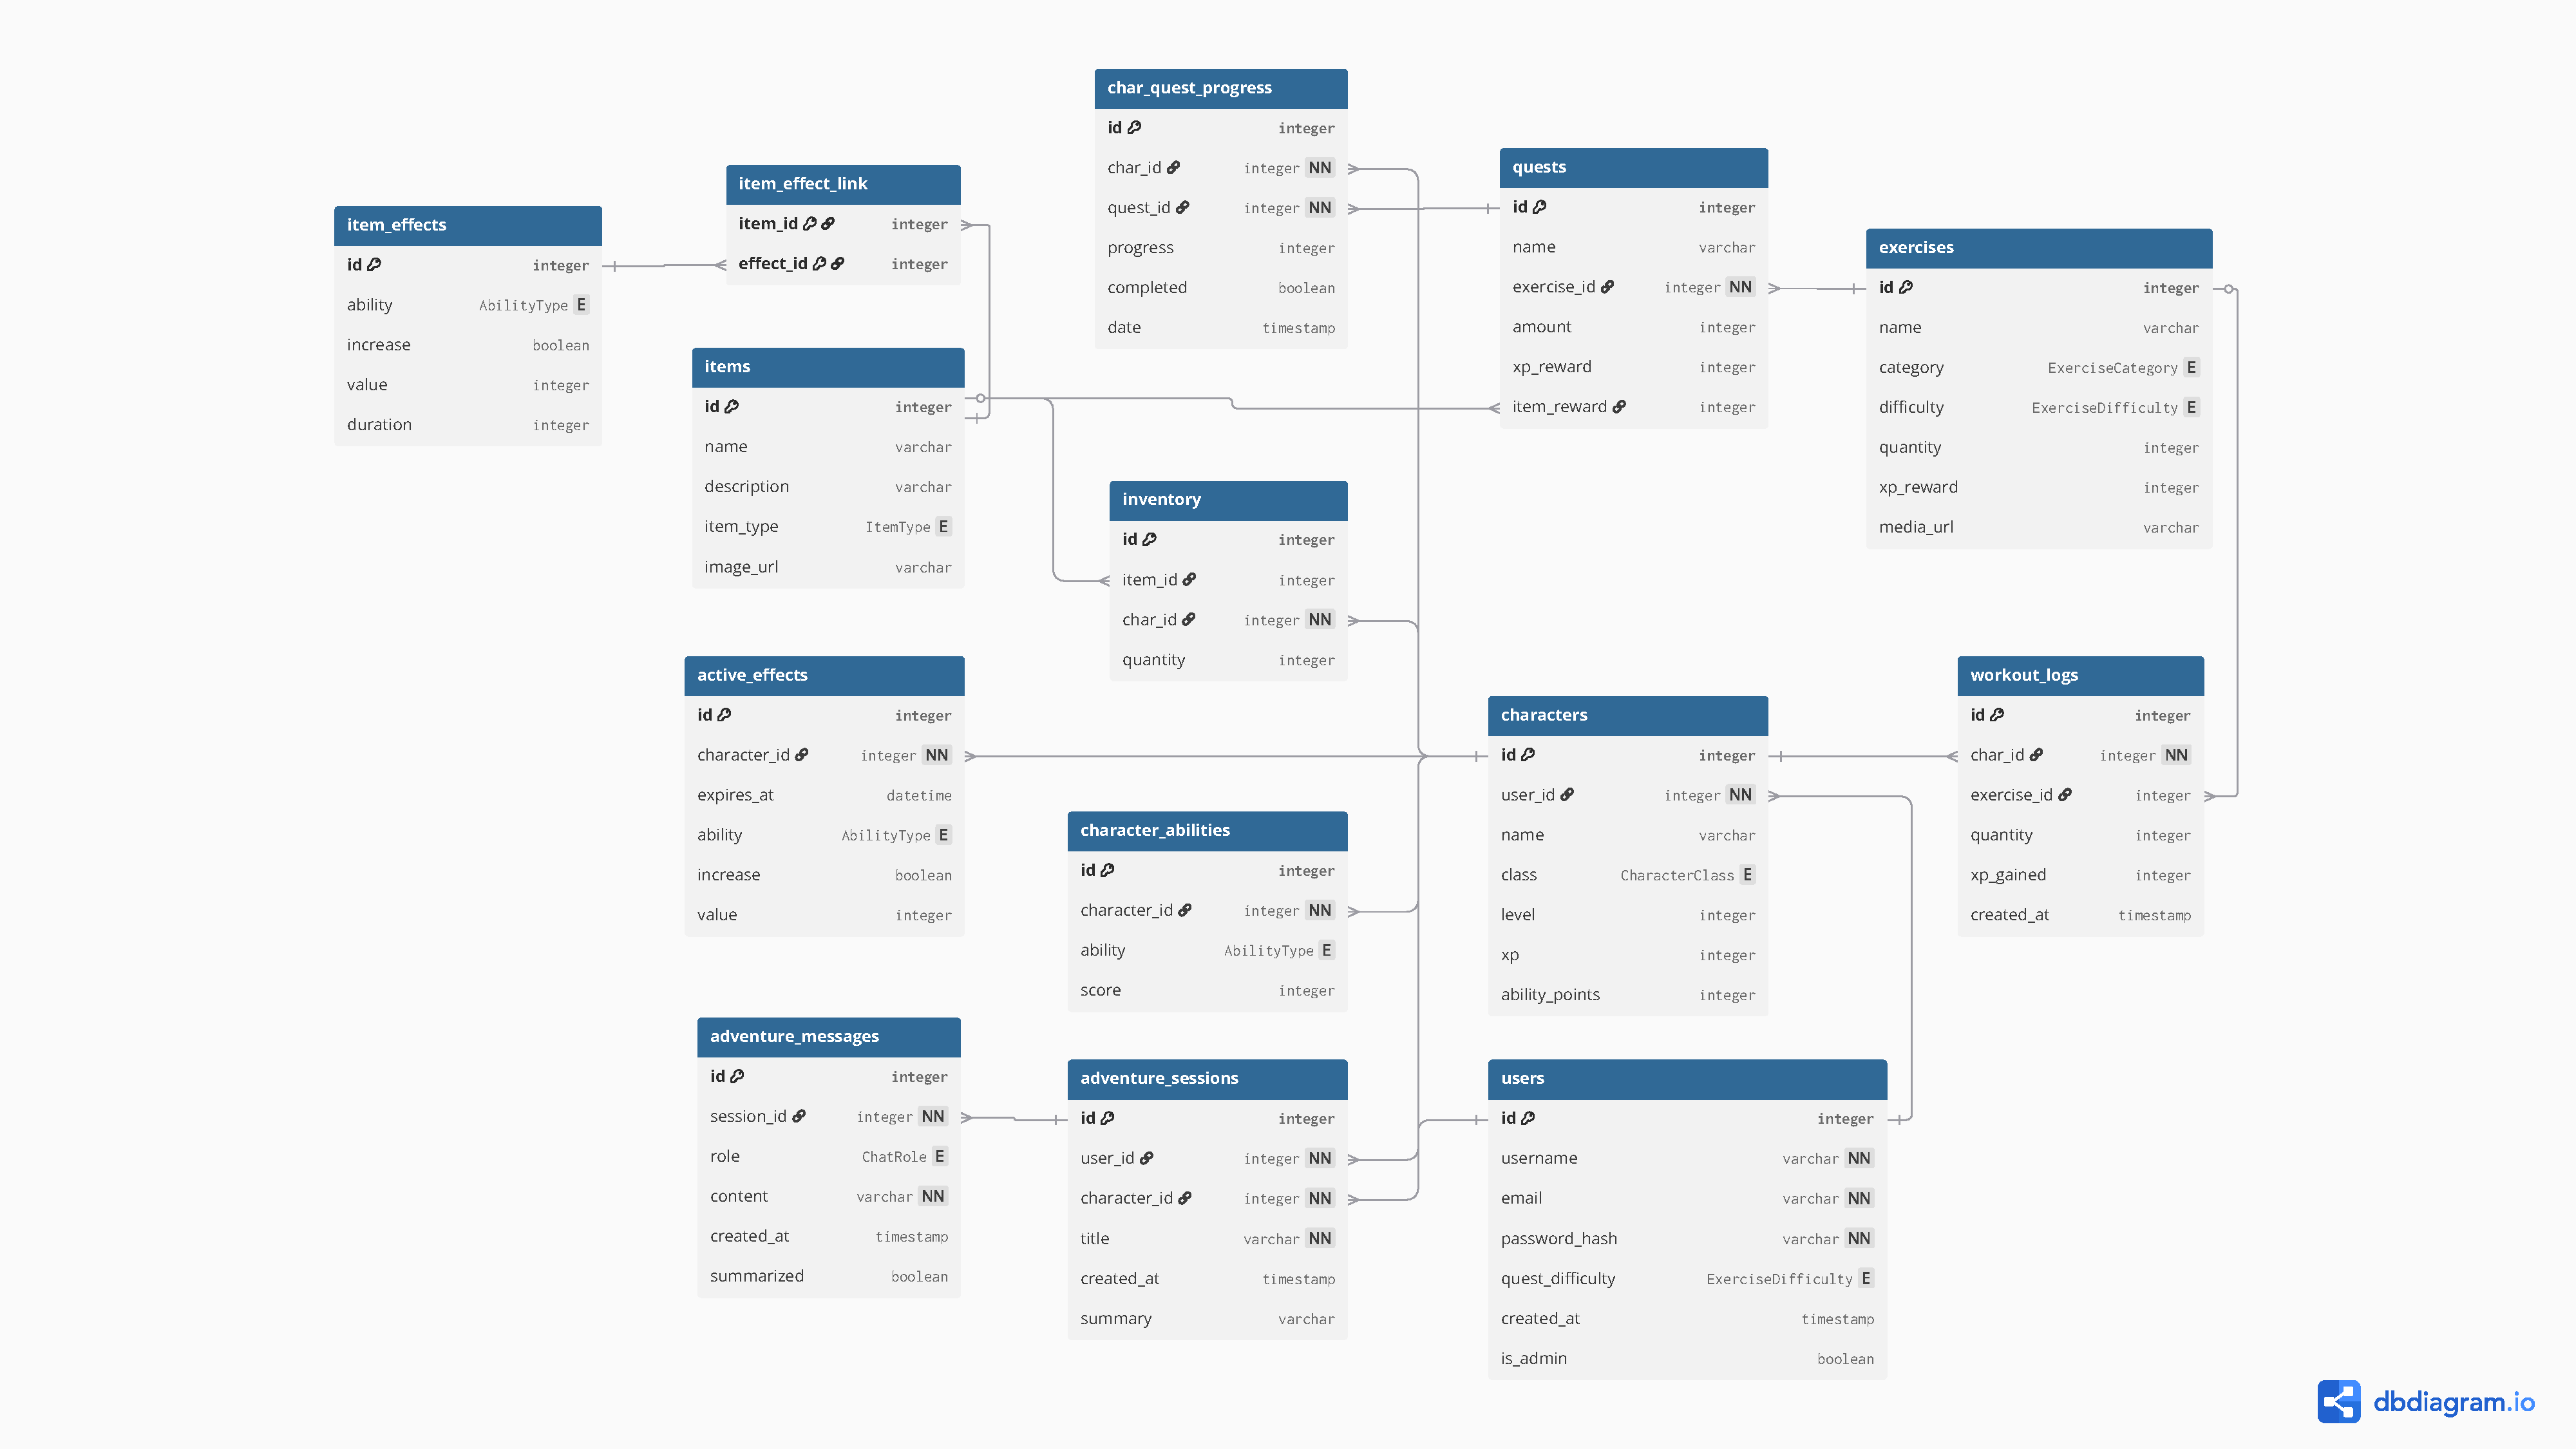
\includegraphics[width=\linewidth]{assets/db.pdf}
    \caption{Az adatbázis modellje. \\ Készült a \url{dbdiagram.io} oldalon~\cite{dbdiagram}. }
    \label{fig_db}
\end{figure}

\subsection{Az adatbázis táblái}

\begin{itemize}

    \item 
    A \textbf{users} tábla a rendszer felhasználóit tárolja, beleértve az azonosító adatokat, bejelentkezési információkat és egyéb felhasználói beállításokat.

    \item 
    A \textbf{characters} tábla a felhasználókhoz tartozó játékbeli karaktereket reprezentálja.

    \item 
    A \textbf{character\_abilities} tábla a karakterek képességeit tárolja. Egy karakterhez több képesség tartozik, és minden képesség külön rekordként jelenik meg.

    \item 
    Az \textbf{exercises} tábla az elérhető edzéseket tartalmazza, beleértve azok kategóriáját, nehézségét és az elérhető jutalmakat.

    \item 
    A \textbf{quests} tábla az edzésekből származtatott napi küldetéseket reprezentálja, amelyek egy adott edzéshez kapcsolódnak.

    \item 
    A \textbf{char\_quest\_progress} tábla a karakterek küldetésekben elért előrehaladását tárolja, beleértve a teljesítés állapotát és a haladási értéket.

    \item 
    A \textbf{workout\_logs} tábla a karakterek által elvégzett edzések naplózására szolgál.

    \item 
    Az \textbf{items} tábla a játékban elérhető tárgyakat tartalmazza, azok típusával és leírásával együtt.

    \item 
    Az \textbf{item\_effects} tábla kiváltható ideiglenes hatásokat definiál, mint az attribútum növelés vagy csökkenés.

    \item 
    Az \textbf{active\_effects} tábla a karaktereken aktív, időben korlátozott hatásokat tárolja.

    \item 
    Az \textbf{item\_effect\_link} tábla az \textbf{items} és a \textbf{item\_effects} táblák közötti társításokat tárolja. 

    \item 
    Az \textbf{inventory} tábla a karakterek és a tárgyak közötti kapcsolatot kezeli, amely egy sok-sok kapcsolatot valósít meg.

    \item
    Az \textbf{adventure\_sessions} tábla a felhasználókhoz tartozó kaland beszélgetéseket tárolja.

    \item 
    Az \textbf{adventure\_messages} tábla az egyes beszélgetések üzeneteit tartalmazza, időrendben eltárolva.

\end{itemize}

\subsection{Az adatbázis kapcsolatai}

\begin{itemize}

    \item
    A \texttt{\textbf{characters}} és \textbf{users} táblák között egy egy-több kapcsolat áll fenn, mivel egy felhasználó több karaktert is létrehozhat, azonban egy karakter csak egy felhasználóhoz tartozik.

    \item
    A \texttt{\textbf{character\_abilities}} tábla a \textbf{characters} táblához kapcsolódik egy egy-több kapcsolattal, mivel egy karakterhez több képesség is tartozhat.

    \item 
    A \textbf{quests} és \textbf{exercises} táblák között egy több-egy kapcsolat áll fenn, ahol több küldetés is ugyanarra az edzésre épülhet.

    \item 
    A \textbf{char\_quest\_progress} tábla kapcsolótáblaként működik a \textbf{characters} és \textbf{quests} táblák között, így egy sok-sok kapcsolatot valósít meg.

    \item 
    A \textbf{inventory} tábla szintén kapcsolótábla, amely a \textbf{characters} és \textbf{items} táblák közötti sok-sok kapcsolatot kezeli.

    \item 
    Az \textbf{item\_effect\_link} tábla a \textbf{items} és \textbf{item\_effects} táblák közötti sok-sok kapcsolatot valósítja meg.

    \item
    Az \textbf{adventure\_sessions} tábla a \textbf{users} és \textbf{characters} táblákhoz kapcsolódik, egy felhasználóhoz és karakterhez több session is tartozhat.

    \item 
    Az \textbf{adventure\_messages} tábla az \textbf{adventure\_sessions} táblához kapcsolódik egy egy-több kapcsolatban, mivel egy beszélgetéshez több üzenet tartozik.

\end{itemize}

\section{UML-diagramok, folyamatábrák}

A rendszer működésének szemléltetésére UML diagramok kerültek elkészítésre, amelyek a szoftver különböző komponensei közötti kapcsolatokat és folyamatokat mutatják be. Ezek segítségével jól nyomon követhető a mobilalkalmazás, a backend szolgáltatás és az adatbázis közötti kommunikáció, valamint a főbb működési lépései.

\subsection{Szekvenciadiagram}

\subsubsection{Bejelentkezés és edzés folyamata}

\Aref{fig_uml_sequence}.\ számú ábrán található szekvenciadiagram a bejelentkezési folyamatot, valamint az edzések és küldetések kezelésének folyamatát szemlélteti. A diagram bemutatja a felhasználó, a mobilalkalmazás, a szerver és az adatbázis közötti kommunikációt. Emellett kitér az offline működésre is, amely során az adatok lokálisan tárolódnak, majd internetkapcsolat esetén szinkronizálásra kerülnek a szerverrel.

\begin{figure}[!ht]
    \centering
    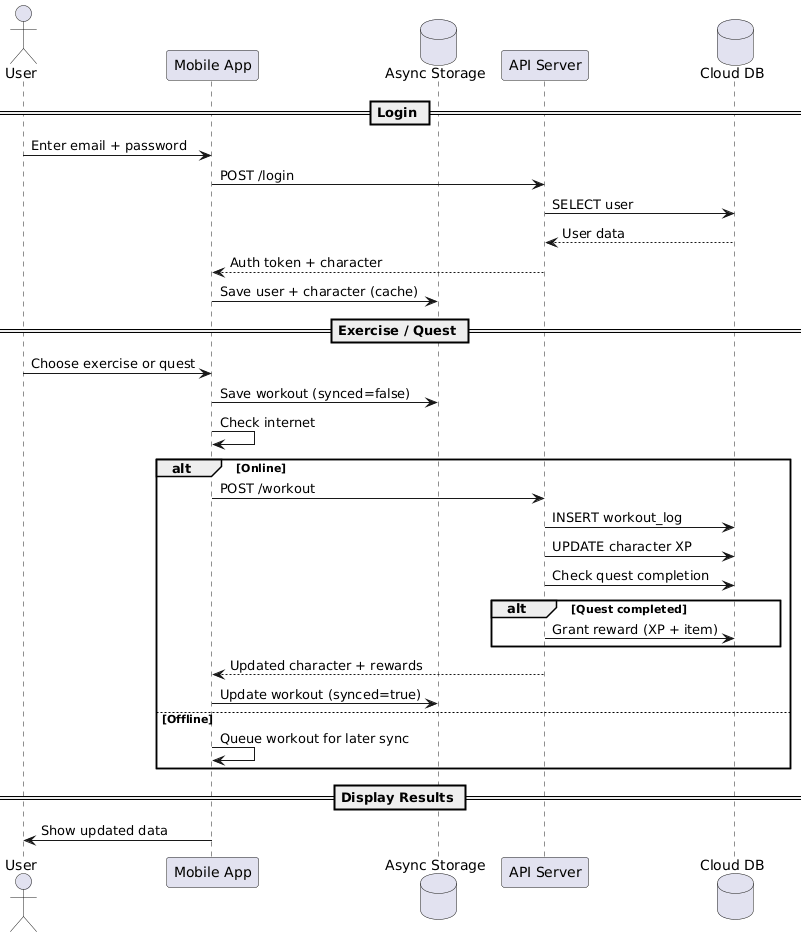
\includegraphics[width=\linewidth]{assets/sequence_diagram.png}
    \caption{Bejelentkezési és edzés folyamat szekvenciadiagramja. \\ Készült a \url{plantuml.com} oldalon~\cite{plantuml}.}
    \label{fig_uml_sequence}
\end{figure}

A bejelentkezés során a felhasználó megadja az e-mail címét és jelszavát, amelyet a program továbbít a backend szerver felé. A szerver lekérdezi a felhasználói adatokat az adatbázisból, majd sikeres azonosítás esetén visszaküldi az autentikációs tokent és a karakterhez tartozó adatokat. Ezek lokálisan is eltárolásra kerülnek gyorsítótár céljából.

Az edzések és küldetések kezelése során a felhasználó kiválaszt egy edzést vagy küldetést. Az alkalmazás eltárolja az edzéshez kapcsolódó adatokat, majd ellenőrzi az internetkapcsolat meglétét. Online működés esetén az edzés adatai feltöltésre kerülnek a szerverre, ahol azok eltárolásra kerülnek, valamint frissül a karakter tapasztalati pontja és szintje. Amennyiben a küldetés teljesül, a rendszer jutalmakat (például XP vagy tárgy) is kioszt. Offline módban az edzés adatai helyben kerülnek eltárolásra, és későbbi szinkronizációra várnak.

A folyamat végén a képernyőn a frissített adatok jelennek meg a
felhasználó számára.

\subsubsection{Egy ,,Kaland'' menete}

\begin{figure}[!ht]
    \centering
    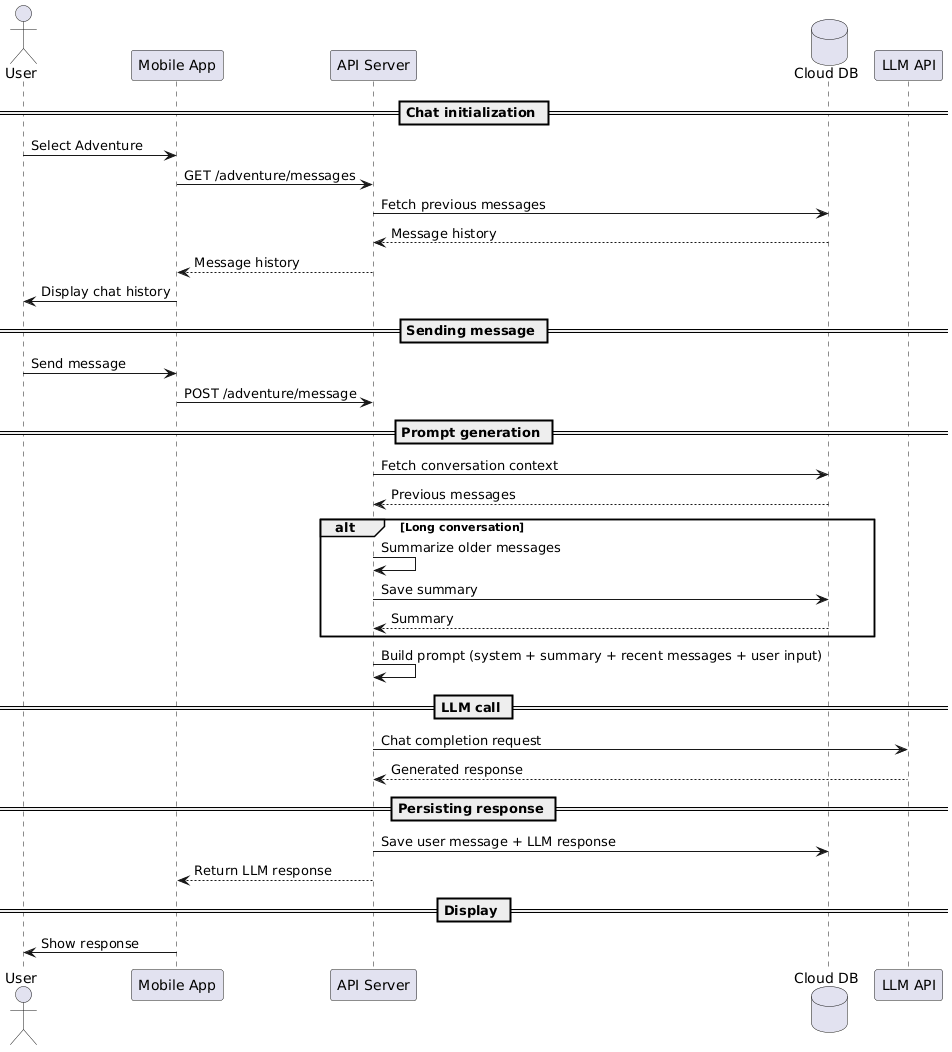
\includegraphics[width=\linewidth]{assets/adventure_sequence.png}
    \caption{LLM alapú chat működésének szekvenciadiagramja. \\ Készült a \url{plantuml.com} oldalon~\cite{plantuml}.}
    \label{fig_uml_chat}
\end{figure}

A rendszer egyik kiemelt funkciója a nagy nyelvi modellen alapuló chat komponens, amely interaktív kalandélményt biztosít a felhasználók számára. \Aref{fig_uml_chat}.\ számú ábrán ennek működési folyamata látható.

A folyamat során a felhasználó kiválaszt egy kalandot, amelyet a mobilalkalmazás a szerveren keresztül kér le. Ezt követően a korábbi üzenetek betöltésre kerülnek az adatbázisból, és megjelenítésre kerülnek a felhasználó számára.

Az új üzenet elküldésekor a program továbbítja a felhasználói inputot a backend szervernek. A szerver összeállítja a modell számára szükséges promptot, amely tartalmazza a rendszerüzenetet, a korábbi beszélgetési előzményeket, valamint az aktuális felhasználói üzenetet. Ezt követően a szerver elküldi a kérést a nagy nyelvi modell API felé.

A modell válasza narratív formában érkezik vissza, amelyet a szerver eltárol az adatbázisban, majd továbbít a frontendnek. Az alkalmazás ezután megjeleníti a választ a felhasználó számára.

\chapter{Saját szoftver megvalósítása}

\section{Az alkalmazás felépítése}

A projekt során alkalmazott technológiák részletes bemutatása a Technológiai áttekintés fejezetben található. Ebben a szakaszban ezen eszközök konkrét felhasználását ismertetem a rendszer megvalósítása során.

\section{Frontend Bemutatása}
A frontend feladata az információk megjelenítése a mobilalkalmazásban,
valamint a backenddel történő kommunikáció.
A frontenden a React Native által biztosított StyleSheeteket használtam a program formázásához. Ezzel egy központi színpalettát is definiáltam és a kódban ezeket használtam, ezáltal biztosítva az egységes megjelenítést. 

Az egyes képernyők külön fájlokban kerültek implementálásra, a felhasználói felület pedig újrafelhasználható komponensekből épül fel, ezekről bővebben \aref{sec_modules}. szekcióban írok.

\section{Backend bemutatása}
A backend feladata a frontendtől érkező kérések feldolgozása, és kommunikáció az adatbázissal, beleértve az adatok lekérdezését és módosítását.

Ahhoz, hogy ezeket elérjük API végpontokat kell definiálni. FastAPI-ban ez könnyen működik, egy példa útvonal látható \aref{code_api_endpoint_examp}.\ számú kódrészleten~\cite{fastapi}.  Az adatlekérdezés az ORM által generált SQL lekérdezéseken keresztül történik, a válaszok pedig JSON formátumban kerülnek visszaadásra~\cite{sqlalchemy}.

A FastAPI automatikusan generál Swagger (OpenAPI) dokumentációt a végpontokhoz, böngészőből történő áttekintését és tesztelését teszi lehetővé~\cite{swagger}. A dokumentáció tartalmazza az elérhető útvonalakat, a bemeneti paramétereket, valamint a válaszok struktúráját is.

A \texttt{/character/has\_haracter/} végponthoz tartozó generált Swagger dokumentáció \aref{fig_swagger_examp}.\ ábrán látható, amely jól szemlélteti az automatikusan előállított interfészt és annak használatát.


\begin{lstlisting}[language=Python, style=pythonstyle, caption={Karakter létezésének lekérdezésre szolgáló végpont}, label={code_api_endpoint_examp}]
@app.get("/has_character/")
def user_has_character(
    current_user: User = Depends(get_current_user), db: Session = Depends(get_db)
):
    logging.info(f"Checking character existence for user_id={current_user.id}")

    character = db.query(Character).filter(Character.user_id == current_user.id).first()

    logging.info(f"Character exists: {bool(character)} for user_id={current_user.id}")
    return {"has_character": bool(character)}
\end{lstlisting}

\begin{figure}[H]
    \centering
    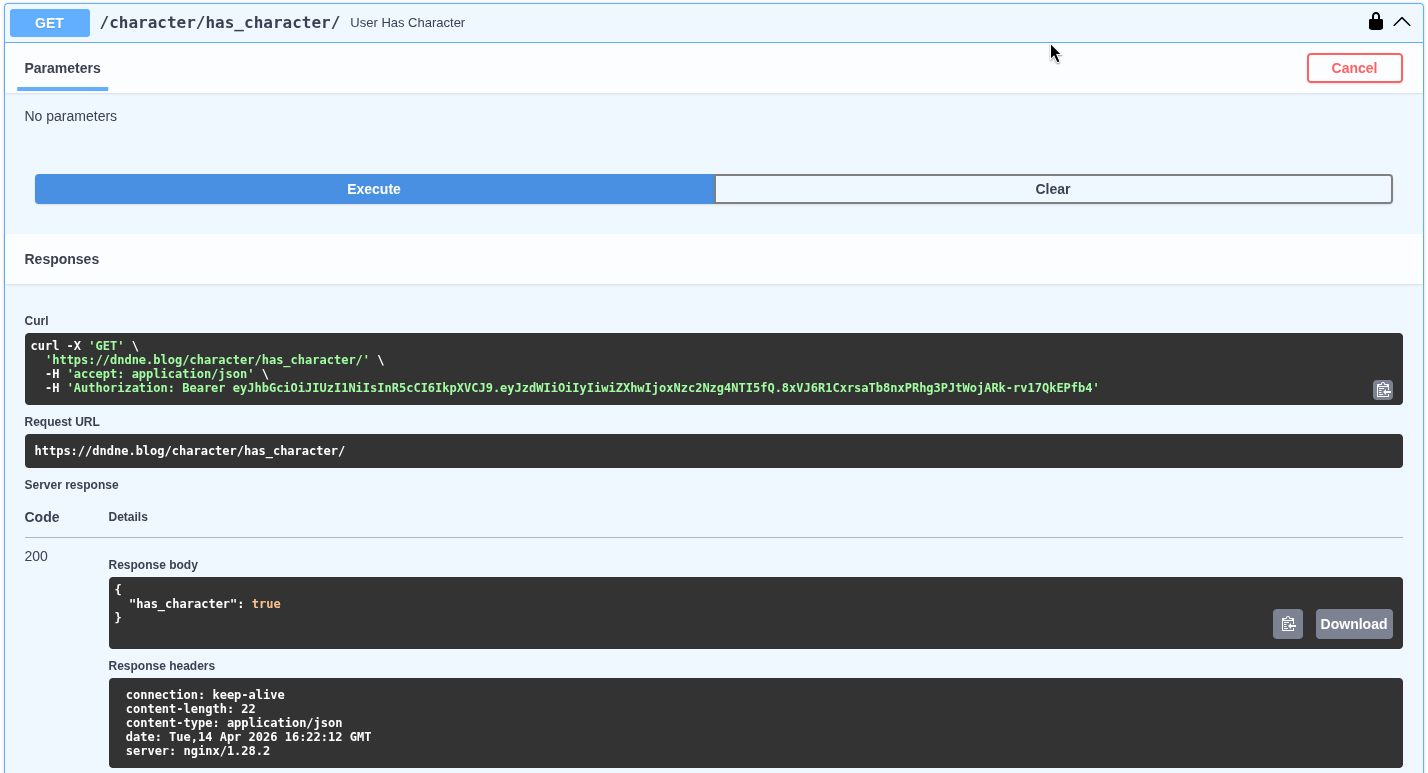
\includegraphics[width=\linewidth]{assets/swagger_exampel.png}
    \caption{FastAPI által generált Swagger/OpenAPI dokumentáció a \texttt{/character/has\_character} végponthoz. \\ (Saját készítésű képernyőkép.)}
    \label{fig_swagger_examp}
\end{figure}

\section{Adatbázis bemutatása}
Az adatbázis PostgreSQL-t használ~\cite{postgresql}, azonban a táblák létrehozását és kezelését a backend végzi az \texttt{SQLAlchemy} ORM könyvtár segítségével~\cite{sqlalchemy}. A Python nyelvben definiált modellek alapján egy SQLAlchemy motor (engine) kerül inicializálásra, amely a backend indulásakor automatikusan létrehozza az adatbázis táblákat.

Ennek megvalósítása \aref{code_db_table_create} kódrészleten látható. Egy példa adatbázis modell \aref{code_inventory_model} kódrészleten kerül bemutatásra. Az adatbázis táblák részletes tervezése \aref{sec_db_plan} szekcióban található.

\begin{lstlisting}[language=Python, style=pythonstyle, caption={Az adatbázis táblák létrehozása SQLAlchemy segítségével}, label={code_db_table_create}]
DATABASE_URL = os.getenv("DATABASE_URL")
if not DATABASE_URL:
    raise RuntimeError("DATABASE_URL environment variable must be set")

engine = create_engine(DATABASE_URL)
SessionLocal = sessionmaker(autocommit=False, autoflush=False, bind=engine)

Base = declarative_base()
Base.metadata.create_all(bind=engine)
\end{lstlisting}

\begin{lstlisting}[language=Python, style=pythonstyle, caption={Az inventory tábla leírása SQLAlchemy modellként}, label={code_inventory_model}]
class Inventory(Base):
    __tablename__ = "inventory"

    id: Mapped[int] = mapped_column(Integer, primary_key=True, index=True)
    item_id: Mapped[int] = mapped_column(ForeignKey("items.id", ondelete="SET NULL"))
    char_id: Mapped[int] = mapped_column(ForeignKey("characters.id", ondelete="CASCADE"))
    quantity: Mapped[int] = mapped_column(Integer)

    item: Mapped["Item"] = relationship("Item")
\end{lstlisting}

A \texttt{items}, \texttt{effects}, \texttt{item\_effect\_links}, \texttt{exercises} és \texttt{quests} táblák feltöltéséhez úgynevezett \emph{seedelést} alkalmaztam. Ennek során JSON formátumú fájlokból kerültek beolvasásra az adatok, amelyeket egy Python script feldolgoz, majd automatikusan feltölti velük az adatbázist.

Ez a megközelítés lehetővé teszi a fejlesztési és tesztelési környezet gyors inicializálását, valamint biztosítja a konzisztens, előre definiált adathalmaz használatát. A seedeléshez használt JSON fájlok a következő GitHub repository-ban érhetők el:
\url{https://github.com/gunicsroland/D-D-Exercise/tree/main/backend/src/services/jsons}

\section{Docker bemutatása}

A rendszer megvalósítása során a fejlesztési környezet egységesítésére konténerizációs megoldást alkalmaztam Docker segítségével~\cite{docker}. A Docker lehetővé teszi az alkalmazás komponenseinek izolált környezetben történő futtatását, ezáltal biztosítva a hordozhatóságot és a reprodukálhatóságot.

A három fő komponensből külön konténerekben futnak:
\begin{itemize}
    \item adatbázis (PostgreSQL~\cite{postgresql})
    \item backend (FastAPI alapú Python alkalmazás~\cite{fastapi})
    \item frontend (React Native / Expo alkalmazás~\cite{react_native,expo})
\end{itemize}

A komponensek együttműködését a Docker Compose konfiguráció biztosítja~\cite{docker_compose}, amely egyetlen konfigurációs fájlban definiálja a szolgáltatásokat, azok hálózati kapcsolatát, valamint az indítási sorrendet.

\subsubsection{Backend konténer}

A backend két Dockerfile segítségével is építhető: egy fejlesztői (\texttt{Dockerfile.dev}) és egy produkciós változat (\texttt{Dockerfile}) is rendelkezésre áll.

A fejlesztői verzió az \texttt{uvicorn} szervert használja, amely alkalmas gyors fejlesztésre és élő újratöltésre. A produkciós verzió ezzel szemben a \texttt{gunicorn} WSGI szervert használja \texttt{uvicorn} workerrel, amely jobb teljesítményt és skálázhatóságot biztosít~\cite{uvicorn,gunicorn}.

A backend konténer indításakor a szükséges Python függőségek telepítésre kerülnek, majd a FastAPI szerver elindul a konfigurált porton.

\subsubsection{Frontend konténer}

A frontend konténer Node.js alapú~\cite{nodejs}, és az Expo keretrendszer segítségével futtatja a React Native alkalmazást webes környezetben. A fejlesztői Dockerfile telepíti a függőségeket, majd elindítja az Expo fejlesztői szervert.

A konténer lehetővé teszi a frontend futtatását böngészőben, hálózaton keresztül elérhető módon, ami megkönnyíti a tesztelést különböző eszközökön.

\subsubsection{Adatbázis konténer}

Az adatbázis PostgreSQL konténerben fut, amely hivatalos Docker image-et használ. Az adatbázis adatai egy Docker volume-ban kerülnek tárolásra, így azok a konténer újraindítása esetén is megmaradnak.

\subsubsection{Docker Compose konfiguráció}

A rendszer komponenseinek indítását a Docker Compose kezeli. A konfigurációs fájl definiálja a három szolgáltatást (db, backend, frontend), valamint azok közötti függőségi kapcsolatokat.

A \texttt{depends\_on} direktíva biztosítja, hogy a backend csak az adatbázis elindulása után induljon el, míg a frontend a backend szolgáltatásra épül.

A környezeti változók \texttt{.env} fájlokból kerülnek betöltésre, amelyek lehetővé teszik a konfiguráció rugalmas kezelését különböző környezetekben.

A teljes rendszer egyetlen parancs segítségével elindítható:
\begin{verbatim}
docker compose up
\end{verbatim}

\section{Modulok bemutatása}
\label{sec_modules}

A szakdolgozat több kisebb modulra bontható, amelyek jól elkülöníthetők egymástól. Ez összhangban van a React szemlélettel, ahol a program komponensekből épül fel. Ezek az egységek nagyrészt megfeleltethetők egy-egy képernyőnek. A backend oldalon az API végpontok is ennek megfelelően kerültek csoportosításra. Ebben a fejezetben ezek működését ismertetem.

\subsection{Autentikációs Modul}

\paragraph{Cél}
A modul feladata a felhasználók hitelesítése és kezelése. Biztosítja az új felhasználók regisztrációját, valamint a meglévő felhasználók bejelentkezését.

\paragraph{Bemenetek és kimenetek}
A bejelentkezéshez felhasználónevet és jelszót fogad a rendszer. Regisztráció esetén email cím megadása is szükséges. Kimenetként egy hitelesítési token kerül visszaadásra.

A token az \texttt{AsyncStorage}-ban~\cite{async_storage} kerül tárolásra, és minden további API hívás során elküldésre kerül a szerver felé hitelesítés céljából.

Az AsyncStorage használata egyszerű és platformfüggetlen megoldást biztosít, azonban nem nyújt titkosított adattárolást, így biztonsági szempontból korlátozott védelmet jelent.

\begin{figure}[!ht]
    \centering
    
\includegraphics[width=\linewidth]{assets/register.png}
    \caption{A regisztrációs felület képe. \\ (Saját készítésű képernyőkép.)}
    \label{fig_register_page}
\end{figure}

\paragraph{Kapcsolódó API végpontok}
\begin{itemize}
    \item \texttt{POST - /auth/register} -- Regisztráció végrehajtása
    \item \texttt{POST - /auth/login} -- Bejelentkezés
\end{itemize}

\paragraph{Megvalósítás részlete}
A biztonságos adattárolás érdekében a jelszavak nem kerülnek közvetlenül eltárolásra, hanem egy hash függvénnyel hashelésre kerülnek. A folyamat során minden jelszóhoz egy véletlenszerűen generált \emph{salt} érték kerül hozzáadásra, amely növeli a biztonságot és megnehezíti az esetleges támadásokat.

A hashelés a \texttt{bcrypt} Python csomag segítségével valósult meg~\cite{bcrypt}. A megvalósítás \aref{code_gen_hash} kódrészleten látható.

\begin{lstlisting}[language=Python, style=pythonstyle, caption={Jelszó hash-elése és ellenőrzése}, label={code_gen_hash}]
def hash_password(password: str) -> str:
    password_bytes = password.encode("utf-8")
    hashed = bcrypt.hashpw(password_bytes, bcrypt.gensalt())
    return hashed.decode("utf-8")

def verify_password(entered_pw: str, hash_pw: str) -> bool:
    entered_pw_bytes = entered_pw.encode("utf-8")
    hashed_bytes = hash_pw.encode("utf-8")
    return bcrypt.checkpw(entered_pw_bytes, hashed_bytes)
\end{lstlisting}

A sikeres bejelentkezés átirányít a felhasználó karakterének oldalára, ha létezik, különben a karakter létrehozása oldalra. Míg a sikeres regisztráció mindig a karakter létrehozás oldalra vezet.

\subsection{Karakter létrehozása modul}

\paragraph{Cél}
A modul célja a felhasználóhoz tartozó D\&D alapú karakter létrehozása. A karakter generálása egy több lépésből álló kérdőív kitöltésével történik, amely a felhasználó fizikai állapotát méri fel.

\paragraph{Bemenetek és kimenetek}
A karakter létrehozásához az alkalmazás több kérdést tesz fel a felhasználónak:

\begin{itemize}
    \item Karakter neve
    \item Karakter kasztja
    \item Mennyi fekvőtámaszt képes elvégezni a felhasználó egy adott időintervallum alatt
    \item Mennyi ideig képes futni megállás nélkül
    \item Mennyire tekinthető hajlékonynak a felhasználó
\end{itemize}

A megadott válaszok alapján kiszámítjuk a karakter hat alap attribútumának (pl. erő, ügyesség, állóképesség stb.) értékét. Egy pontszámításnak az eredménye látható \aref{fig_char_create} ábrán.

A karakter létrehozásának megerősítése után a frontend egy API hívást indít a backend felé, amely elmenti a karaktert az adatbázisban, majd visszaadja annak adatait. Ezt követően a karakter nézetre navigáljuk a felhasználót.

\paragraph{Kapcsolódó API végpontok}
\begin{itemize}
    \item \texttt{POST - /character/} - Karakter létrehozása az adott felhasználónak
\end{itemize}

\begin{figure}[!ht]
    \centering
    
\includegraphics[width=\linewidth]{assets/karakter_create.png}
    \caption{A karakter létrehozása előtti összefoglaló képernyő. \\ (Saját készítésű képernyőkép.)}
    \label{fig_char_create}
\end{figure}

\paragraph{Megvalósítás részlete}

A karakter attribútumainak kiszámítása egy szabályalapú pontszámítási rendszer segítségével történik, amely a felhasználó által megadott fizikai teljesítményt képezi le a játékbeli értékekre. A cél az, hogy a karakter fejlődése közvetlen kapcsolatban álljon a valós edzési aktivitással.

Minden kaszthoz tartozik egy alap attribútumeloszlás ($baseStats$), amely meghatározza a karakter kiindulási értékeit. Ezt az alapeloszlást módosítják a felhasználó válaszai alapján számított bónuszértékek.

Az egyes attribútumok végső értékei az alábbi képlet szerint kerülnek meghatározásra:

\[
stat = clamp(baseStat + bonus, 1, 20)
\]

ahol a $clamp$ függvény biztosítja, hogy az attribútumok értékei egy előre definiált intervallumba essenek:

\[
clamp(x, min, max) = \max(min, \min(max, x))
\]

\paragraph{Bónuszértékek meghatározása}

A bónuszok a bemeneti értékek normalizálásával kerülnek kiszámításra:

\begin{itemize}
    \item \textbf{Erő (Strength):}
    \[
    bonus_{str} = \left\lfloor \frac{pushups}{15} \right\rfloor
    \]

    \item \textbf{Állóképesség (Constitution):}
    \[
    bonus_{con} = \left\lfloor \frac{runTime}{60} \right\rfloor
    \]

    ahol a $runTime$ másodpercben értendő.

    \item \textbf{Ügyesség (Dexterity):}
    \[
    bonus_{dex} = \left\lfloor \frac{agility}{5} \right\rfloor
    \]
\end{itemize}

A további attribútumok (intelligencia, bölcsesség, karizma) jelenleg nem kerülnek módosításra, kizárólag a kaszthoz tartozó alapértékekből származnak.

\paragraph{Korlátok és normalizálás}

Az attribútumok értéke az $[1, 20]$ intervallumba van korlátozva, amely megfelel a D\&D által alkalmazott értéktartománynak. A korlátozás biztosítja, hogy a rendszer stabil maradjon szélsőséges bemeneti értékek esetén is.

\paragraph{Értelmezés}

A választott leképezés célja, hogy a fizikai teljesítmény és a játékbeli karakterjellemzők között intuitív kapcsolat alakuljon ki:
\begin{itemize}
    \item a fekvőtámaszok száma az erő attribútumot növeli,
    \item a futással töltött idő az állóképességet befolyásolja,
    \item a hajlékonyság az ügyességet javítja.
\end{itemize}

A modell lineáris felépítésű, amely egyszerű implementációt és könnyű értelmezhetőséget biztosít. Ugyanakkor a rendszer később tovább bővíthető komplexebb, például nemlineáris vagy súlyozott számítási módszerekkel.

\subsection{Karakter modul}

\paragraph{Cél}
A karakter modul feladata a felhasználóhoz tartozó játékbeli karakter megjelenítése és kezelése. Biztosítja a karakter adatainak (név, szint, tapasztalati pontok, képességek) vizualizációját, valamint lehetőséget ad a karakter fejlesztésére és módosítására.

\paragraph{Bemenetek és kimenetek}
A backend API-ból lekért karakter adatokat használja bemenetként. Ezek közé tartozik a karakter neve, szintje, tapasztalati pontjai, képességpontjai és aktív hatásai.

A felhasználói interakciók (például képesség fejlesztése vagy névváltoztatás) API hívásokat indítanak a backend felé. A válaszok alapján a frontend frissíti a karakter állapotát.

\begin{figure}[!ht]
    \centering
    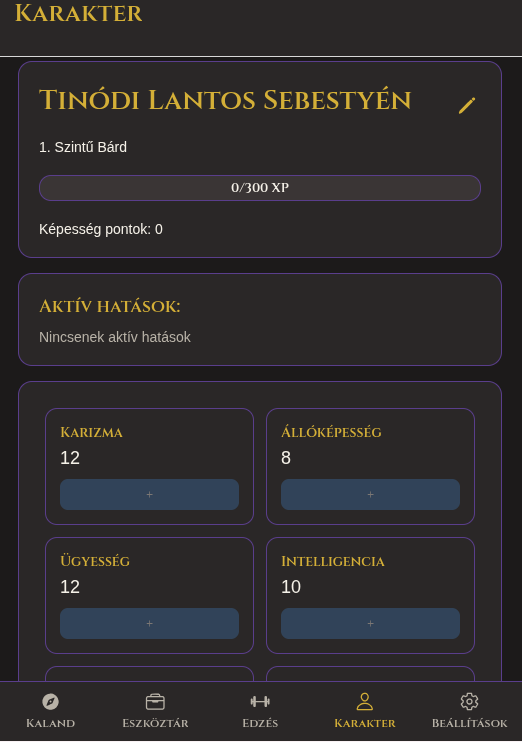
\includegraphics[width=\linewidth]{assets/karakter.png}
    \caption{A Karakter oldal nézete. \\ (Saját készítésű képernyőkép.)}
    \label{fig:placeholder}
\end{figure}

\paragraph{Kapcsolódó API végpontok}
\begin{itemize}
    \item \texttt{GET - /character/} - Adott felhasználó első karakterét adja vissza. 
    \item \texttt{PUT - /character/upgrade\_ability} - A jelenlegi karakter egy attribútumának fejlesztése
\end{itemize}

\paragraph{Megvalósítás részlete}
A karakter nézet egy React Native képernyőként valósul meg, amely több kisebb komponensből épül fel. Az állapotkezelés Context API segítségével történik, amely biztosítja, hogy a karakter adatai az alkalmazás több pontján is elérhetőek legyenek.

A felhasználó lehetőséget kap a karakter nevének módosítására egy modal ablak segítségével~\cite{react_modal}. A módosítás során a frontend validálja a bemenetet, majd API hívást indít a backend felé. Sikeres válasz esetén a karakter adatai újratöltésre kerülnek.

A képességek fejlesztése szintén API híváson keresztül történik, amely során a backend ellenőrzi a rendelkezésre álló képességpontokat, majd frissíti az adatbázist.

Az egység valós időben frissíti az aktív hatásokat egy időalapú hook segítségével. Ezzel biztosítva, hogy pontosan mutatja a karakter attribútumainak értékét és az aktív hatásokból visszamaradó időket.

\subsection{Kaland modul}

\paragraph{Cél}

A kaland modul feladata a felhasználók által létrehozott kalandok (session-ök) kezelése. Lehetővé teszi új kalandok indítását, a meglévő kalandok listázását, kiválasztását, átnevezését és törlését. Biztosítja a chat alapú kalandok keretrendszerét.

\paragraph{Bemenetek és kimenetek}

A modul bemenetként az alábbi adatokat kezeli:
\begin{itemize}
    \item Új kaland címe
    \item Kaland azonosító (kiválasztás, törlés, módosítás esetén)
\end{itemize}

Kimenetként a rendszer:
\begin{itemize}
    \item A felhasználóhoz tartozó kalandok listáját adja vissza
    \item A létrehozott vagy módosított kaland adatait
\end{itemize}

\paragraph{Kapcsolódó API végpontok}
\begin{itemize}
    \item \texttt{GET /adventure/} – kalandok listázása
    \item \texttt{POST /adventure/start} – új kaland létrehozása
    \item \texttt{DELETE /adventure/\{id\}} – kaland törlése
    \item \texttt{PUT /adventure/\{id\}/title} – kaland átnevezése
\end{itemize}

\paragraph{Megvalósítás részlete}

A frontend oldalon az elkezdett kalandok egy lista alapú felületként jelennek meg, ahol a felhasználó megtekintheti őket, valamint újat indíthat. A kiválasztott kaland egy külön chat felületre navigál.

\subsection{Chat modul}

\paragraph{Cél}

A chat modul feladata a felhasználó és egy nagy nyelvi modell (Large Language Model) közötti kommunikáció megvalósítása. Biztosítja az interaktív, szöveges alapú kalandélményt, ahol a modell Dungeon Master szerepben narrálja a történetet.

\paragraph{Bemenetek és kimenetek}

A modul bemenetként:
\begin{itemize}
    \item Felhasználói üzeneteket
    \item A kiválasztott kalandhoz tartozó előzményeket
\end{itemize}

Kimenetként:
\begin{itemize}
    \item A modell által generált válaszokat (narráció)
    \item Frissített beszélgetési előzmény
\end{itemize}

\paragraph{Kapcsolódó API végpontok}
\begin{itemize}
    \item \texttt{GET /messages/\{session\_id\}} – üzenetek lekérése az adott kalandhoz
    \item \texttt{POST /messages/\{session\_id\}} – új üzenet küldése az adott kalandhoz
\end{itemize}

\subsubsection{Megvalósítás részlete}

A komponens  a Google Gemini nyelvi modell API-ját használja a válaszok generálására~\cite{gemini_api}. A backend feladata, hogy a felhasználói üzenetekből és a korábbi beszélgetésből egy strukturált promptot állítson elő. Egy példa prompt található \aref{code_prompt_basic} kódrészlet, illetve egy válasz \aref{fig_chat_example} ábrán.

A prompt több komponensből épül fel:
\begin{itemize}
    \item rendszer prompt (Dungeon Master szerep, szabályok)
    \item karakter adatai (név, kaszt, szint, képességek)
    \item korábbi üzenetek
    \item opcionálisan a korábbi történések összefoglalója
    \item aktuális felhasználói input
\end{itemize}

\paragraph{Összefoglalás készítés feltételei}

Az összefoglalás készítése akkor történik meg, ha a még nem összefoglalt üzenetek száma meghaladja a \texttt{SUMMARY\_TRIGGER\_MESSAGES} konstansban megadott értéket.

Az összefoglalás során:
\begin{itemize}
    \item csak a még nem összefoglalt üzenetek kerülnek feldolgozásra
    \item az összefoglaló szöveg külön mezőben kerül eltárolásra az adatbázisban
\end{itemize}

A rendszer nem az összes üzeneten végez egy összegzést, hanem a korábbi összefoglalót kiegészíti, így biztosítva a kontextus folytonosságát és csökkentve a feldolgozási költséget. A prompt összeállításakor az összefoglaló mellett csak a legutóbbi \texttt{RECENT\_MESSAGES\_TO\_KEEP} darab üzenetet veszi figyelembe. Ez a megközelítés biztosítja, hogy a modell elegendő friss kontextust kapjon, miközben a tokenfelhasználás kontroll alatt marad.

\paragraph{Chat feldolgozási folyamat pszeudokódja}

\Aref{code_chat_flow} pszeudokód összefoglalja a chat modul teljes feldolgozási folyamatát.

\begin{lstlisting}[style=pseudostyle, caption={Chat üzenet feldolgozási folyamat}, label={code_chat_flow}]
FÜGGVÉNY generate_dm_response(session, user_message, db):
    messages <- lekérdezés(session.id)
    
    HA messages.száma > SUMMARY_TRIGGER_MESSAGES:
        session.summary <- summarize(messages, session.summary)

    system_prompt <- karakter adatok + Dungeon Master szerep

    contents <- []
    contents.hozzáad(system_prompt)

    HA session.summary létezik:
        contents.hozzáad(session.summary)

    recent_messages <- utolsó RECENT_MESSAGES_TO_KEEP üzenet
    contents.hozzáad(recent_messages)

    contents.hozzáad(user_message)

    response_stream <- LLM.generate_stream(contents)

    full_response <- ""

    CIKLUS chunk IN response_stream:
        full_response <- full_response + chunk
        visszaküld chunk

    ment(user_message)
    ment(full_response)

    VISSZA full_response
END
\end{lstlisting}

\paragraph{Hibakezelés és stabilitás}

A rendszer több ponton tartalmaz hibakezelési mechanizmusokat:

\begin{itemize}
    \item a válasz generálása streaming módban történik, amely lehetővé teszi a folyamatos megjelenítést
    \item streaming hiba esetén a rendszer fallback mechanizmust alkalmaz, és a teljes választ egyben próbálja feldolgozni
    \item ha a válasz nem megfelelő formátumú (pl. nem JSON), a rendszer szövegként kezeli azt
    \item tartós hiba esetén a felhasználó hibaüzenetet kap
\end{itemize}

A beszélgetések konzisztenciájának biztosítása érdekében minden üzenet mentésre kerül, így hiba esetén a folyamat újraindítható.

\paragraph{Minőségbiztosítás}

A generált válaszok minőségének biztosítása érdekében az alábbi szempontok kerülnek figyelembevételre:
\begin{itemize}
    \item a rendszer prompt explicit módon meghatározza a modell szerepét (Dungeon Master)
    \item a válasz nyelve és stílusa előre rögzített
    \item a beszélgetési előzmények biztosítják a kontextus folytonosságát
\end{itemize}

A fejlesztés során manuális teszteléssel ellenőriztem, hogy a modell válaszai konzisztensen követik a megadott szerepet és narratív stílust.

\begin{figure}[!ht]
        \centering
        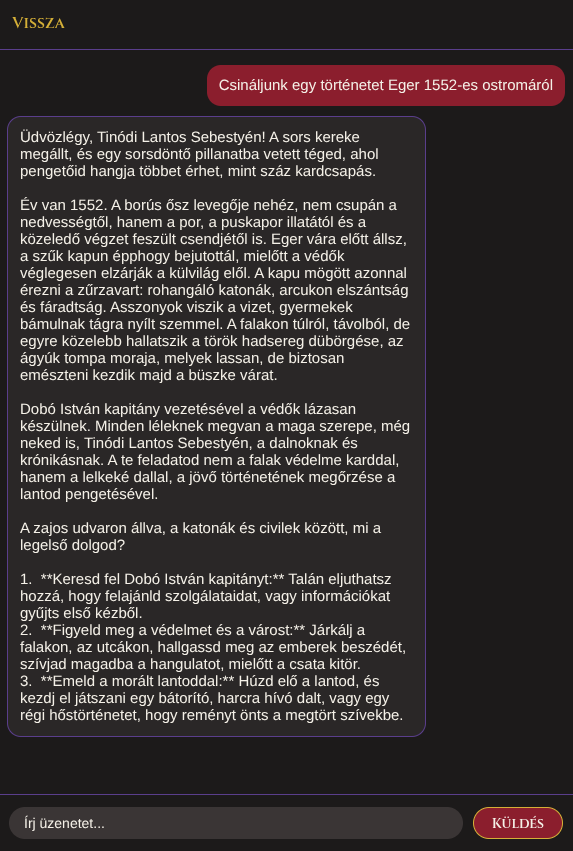
\includegraphics[width=\linewidth]{assets/chat.png}
        \caption{Példa beszélgetés \\ (Saját készítésű képernyőkép)}
        \label{fig_chat_example}
\end{figure}

\begin{lstlisting}[style=textstyle, caption={Egy példa prompt összegzés nélkül}, label={code_prompt_basic}, xleftmargin=0cm, xrightmargin=0cm]
[
  {
    role: "user",
    content: "
    You are a Dungeon Master.
    The player character is:
    Name: Tinódi Lantos Sebestyén
    Class: Bard
    Level: 1
    Abilities: strength: 6, dexterity: 12, constitution: 8,
               intelligence: 10, wisdom: 10, charisma: 12

    Respond in immersive D&D style.
    It is a simplified game, we don't have items or spells.
    Respond in Hungarian.
    "
  },
  {
    role: "user",
    content: "Csináljunk egy történetet Eger 1552-es ostromáról"
  },
  {
    role: "model",
    content: "Üdvözlégy, Tinódi Lantos Sebestyén! ..." (a modell által generált narráció)
  },
]
\end{lstlisting}

\subsection{Edzés modul}


Az edzés modul a legfontosabb része az alkalmazásnak, ezért egyben a legösszetettebb is. A következő képen épül fel:
\begin{itemize}
    \item Edzések képernyő
    \begin{itemize}
        \item Napi küldetések
        \item Meglévő edzések
    \end{itemize}
    \item Edzésterv megcsinálása
\end{itemize}

\subsubsection{Edzések képernyő}

\paragraph{Cél}
Az edzések képernyő célja, hogy a felhasználó számára áttekinthető módon megjelenítse az elérhető edzéseket, valamint az aktuális napi küldetéseket. A felület lehetőséget biztosít arra, hogy a felhasználó kiválassza és összeállítsa saját edzéstervét, amely később végrehajtható.

\paragraph{Bemenetek és kimenetek}

A modul bemenetként:
\begin{itemize}
    \item A felhasználó által kiválasztott szűrőket (kategória, nehézség)
    \item A felhasználó által kiválasztott napi küldetés nehézségi szintet
\end{itemize}

Kimenetként:
\begin{itemize}
    \item A felhasználó aktuális napi küldetései
    \item Küldetés előrehaladás (progress)
    \item Szűrt és rendezett edzéslista
\end{itemize}

\paragraph{Kapcsolódó API végpontok}

\begin{itemize}
    \item \texttt{GET /exercises/} – elérhető edzések lekérése
    \item \texttt{GET /quests/daily\_quests} – napi küldetések lekérése
    \item \texttt{GET /quests/quest\_progress} – küldetés előrehaladás lekérése
    \item \texttt{PUT /character/quest\_difficulty} – nehézségi szint módosítása
\end{itemize}

\paragraph{Megvalósítás részletei}

A képernyő két fő részre oszlik: a napi küldetések megjelenítésére, valamint az edzések listájára. A napi küldetések esetében a felhasználó kiválaszthatja a kívánt nehézségi szintet, amely hatással van a generált feladatokra és a megszerezhető jutalmakra.

Az edzések listája dinamikusan szűrhető kategória és nehézség alapján, valamint rendezhető különböző szempontok szerint. Ez lehetővé teszi a felhasználó számára, hogy személyre szabott edzéstervet állítson össze.

A napi küldetéseknél és az edzések listánál is lehetőség van, hogy hozzáadjuk őket az edzéstervünkhöz, amit végre szeretnénk hajtani. Ennek vezérlése az \texttt{ExerciseContext} segítségével történt, így a napi küldetéseket és egy edzés megjelenését egyszerűen ki lehetett egy komponensbe refaktorálni. Ennek egy részleges megvalósítása látható \aref{code_exercise_context} kódrészleten. A Context teljes megvalósítása a forráskódban található (\url{https://github.com/gunicsroland/D-D-Exercise/blob/main/frontend/src/context/GameContext.tsx}).

\begin{lstlisting}[language=TypeScript, style=typescriptstyle, caption={Exercise Context az edzésterv kezelése (részlet)}, label={code_exercise_context}]
    const addExercise = (ex: Exercise) => {
    const newPlan: ExercisePlan = {
      exercise: ex,
      uuid: Date.now() + Math.random(),
    };

    setPlan((prev) => [...prev, newPlan]);
  };

  const removeExercise = (uuid: number) => {
    setPlan((prev) => prev.filter((e) => e.uuid !== uuid));
  };

  const clearPlan = () => setPlan([]);

  const startPlan = () => {
    router.push("/exerciseRunner");
  };
\end{lstlisting}

Az edzésterv elindításához az oldalon egy abszolút pozícióval rendelkező gomb található, amely a kiválasztott edzéseket tartalmazó terv végrehajtását indítja el.

\subsubsection{Edzésterv teljesítése}

\paragraph{Cél}
Egy oldal, ahol egymás után lehet az edzéstervhez hozzáadott feladatokat végrehajtani. Minden feladat között egy kis szünet található. A kivitelezéshez a \emph{Home Workout - No Equipment} nevű telefonos alkalmazást vettem alapul~\cite{home_workout}

\paragraph{Bemenetek és kimenetek}
A modul bemenetként:
\begin{itemize}
    \item A felhasználó által összeállított edzéstervet
    \item A felhasználó interakcióit (pl. következő, előző, befejezés)
\end{itemize}

Kimenetként:
\begin{itemize}
    \item Az aktuális gyakorlat megjelenítése
    \item Az edzés előrehaladásának visszajelzése
    \item A befejezett gyakorlatok elküldése a szerver felé
\end{itemize}

\paragraph{Kapcsolódó API végpontok}

\begin{itemize}
    \item \texttt{POST /exercise/finish/\{exercise\_id\}} – egy gyakorlat teljesítésének rögzítése
\end{itemize}

\paragraph{Megvalósítás részletei}

A modul lineáris folyamatként kezeli az edzéstervet. Az aktuális gyakorlatot egy index változó határozza meg, a már teljesített feladatokat pedig egy halmazban (\texttt{Set}) tároljuk a duplikációk elkerülése végett. A gyakorlatok között egy visszaszámlálóval jelzett pihenőidő található, amelynek lejárta után a rendszer automatikusan a következő feladatra lép.

\paragraph{Edzés lezárása}

Az edzés befejezésekor a rendszer végigiterál a teljesített gyakorlatokon, és egyesével elküldi azokat a backend felé. Hálózati hiba esetén a rendszer a gyakorlatokat egy perzisztens, AsyncStorage alapú sorba (queue) menti.

A backend által végrehajtott lépések \aref{code_exercise_finish} pszeudokód szemlélteti.

\begin{lstlisting}[style=pseudostyle, caption={Edzés teljesítésének feldolgozása}, label={code_exercise_finish}]
FÜGGVÉNY finish_exercise (exercise_id : int, user: User):

    exercise <- LEKÉRÉS ADATBÁZISBÓL

    HA exercise NEM LÉTEZIK:
        VISSZA 404 hiba

    HA user-nek nincs karaktere:
        VISSZA 404 hiba

    character <- user első karaktere

    // 1. XP hozzáadás
    add_xp(character.id, exercise.xp_reward)

    // 2. Napi questek kezelése
    daily_quests <- napi questek lekérése

    CIKLUS minden quest IN daily_quests:
        HA quest.exercise_id == exercise_id:
            update_quest_progress(character.id, quest.id)

            // ha quest teljesül:
            // -> jutalmak kiosztása (XP + item)
    
    // 3. Edzés logolása
    log_exercise_completion(character.id, exercise_id, exercise.xp_reward, exercise.quantity)

    VISSZA sikeres válasz
END

\end{lstlisting}

A lezárását követően a lokális edzésterv törlésre kerül, és a felhasználó visszairányításra kerül a korábbi nézetre, miközben a játékállapot frissül.


\paragraph{Offline szinkronizáció és konzisztencia}

A szinkronizáció automatikusan történik, amikor a kliens újra hálózati kapcsolatot észlel. A rendszer ilyenkor sorban végigiterál a tárolt elemeken, és megkísérli azok elküldését a szerver felé.

Sikeres feldolgozás esetén az adott elem eltávolításra kerül a sorból, míg sikertelen kérés esetén a sorban marad. Ez biztosítja, hogy csak a nem feldolgozott elemek kerüljenek újraküldésre.

\textbf{Hibakezelés}

A szinkronizáció során:
\begin{itemize}
    \item sikertelen kérés esetén az adott elem a sorban marad
    \item részleges siker esetén csak a hibás elemek kerülnek újrapróbálásra
    \item a szinkronizáció automatikusan újraindul hálózati kapcsolat helyreállásakor
\end{itemize}

Ez a megközelítés biztosítja az adatok megőrzését átmeneti hálózati hibák esetén.  Ennek a működésnek egy részlete \aref{code_exercise_sync} kódrészleten látható.

 \begin{lstlisting}[language=TypeScript, style=typescriptstyle, caption={Az edzések elmentése és szinkronizálása (részlet)}, label={code_exercise_sync}]
     
export async function finishExercise(token: string, id: number) {
  try {
    const res = await fetch(`${API_URL}/exercises/finish/${id}`, {
      method: "POST",
      headers: {
        "Content-Type": "application/json",
        Authorization: `Bearer ${token}`,
      },
    }); ...
}

export async function syncFinishedExercises(token: string) {
  const queue = await getOfflineCompletions();

  ...

  for (const item of queue) {
    try {
      const res = await fetch(
        `${API_URL}/exercises/finish/${item.exerciseId}`,
        {
          method: "POST",
          headers: {
            "Content-Type": "application/json",
            Authorization: `Bearer ${token}`,
          },
        },
      );
    }
    ...
  }
}
 \end{lstlisting}

\section{Futtatási leírás}

Az alkalmazás lokális futtatása Docker segítségével történik, amely biztosítja a teljes rendszer (adatbázis, backend és frontend) egyszerű és egységes indítását. A projekt tartalmaz egy \texttt{docker-compose.yml} fájlt, amely definiálja a szükséges szolgáltatásokat és azok konfigurációját.

A rendszer több, különálló \texttt{.env} fájlt használ a különböző komponensek (backend, frontend, illetve adatbázis) konfigurálására. A teljes konfiguráció a forráskódtárban található példa \texttt{.env} fájlok alapján reprodukálható.

A \ref{code_env} példa egy leegyszerűsített, aggregált konfigurációt mutat be, amely szemlélteti a rendszer működéséhez szükséges főbb környezeti változók típusait. Fontos megjegyezni, hogy a példában szereplő értékek demonstrációs célt szolgálnak, és nem tekinthetők biztonságos konfigurációnak.

\begin{lstlisting}[style=textstyle, caption={Példa .env konfiguráció}, label={code_env}]
# Általános portok
BACKEND_PORT=8000
FRONTEND_PORT=8081

# Adatbázis
POSTGRES_DB=dndne
POSTGRES_USER=dndne_admin
POSTGRES_PASSWORD=admin
POSTGRES_PORT=5432
DATABASE_URL=

# API és CORS
EXPO_PUBLIC_API_URL=https://dndne.blog
CORS_ORIGINS=*

# Autentikáció és biztonság
ADMIN_API_KEY=supersecret
SECRET_KEY=supersecret123456
ALGORITHM=HS256
ACCESS_TOKEN_EXPIRE_MIN=10080

# AI modell
MODEL_NAME=gemini-2.5-flash
GEMINI_API_KEY=api_key
\end{lstlisting}

A rendszer indítása az alábbi parancsokkal történik:

\begin{verbatim}
docker compose up --build
\end{verbatim}

A parancs hatására:
\begin{itemize}
    \item elindul a PostgreSQL adatbázis konténer,
    \item elindul a backend FastAPI alkalmazás,
    \item elindul a frontend Expo alkalmazás,
    \item valamint a szükséges hálózati kapcsolatok automatikusan konfigurálásra kerülnek.
\end{itemize}

A konténerek elindítása után az alkalmazás komponensei a konfigurált portokon keresztül érhetők el:
\begin{itemize}
    \item backend: \texttt{http://localhost:8000}
    \item frontend: \texttt{http://localhost:8081}
\end{itemize}

\chapter{Tesztelés}

A rendszer megbízhatóságának biztosítása érdekében a fejlesztés során kiemelt figyelmet fordítottam a tesztelésre. A tesztelés célja nem csupán a kód lefedettségének növelése volt, hanem a funkcionális követelmények teljesülésének igazolása, valamint a kritikus felhasználói folyamatok helyes működésének ellenőrzése.

A tesztelés során a funkcionális követelmények és a tesztesetek között megfeleltetést alakítottam ki, amely biztosítja a követelmények nyomon követhetőségét (traceability). A rendszer tesztelése frontend és backend szinten történt, egység- és integrációs tesztekkel kiegészítve.

A teszteredmények összefoglalását az 
\ref{tab_auth_tests}, 
\ref{tab_char_create_tests}, 
\ref{tab_char_tests}, 
\ref{tab_adventure_tests}, 
\ref{tab_chat_tests} 
és \ref{tab_workout_tests} táblázatok tartalmazzák.

\section{Autentikációs modul tesztelése}

\begin{table}[h]
\centering
\begin{tabularx}{\textwidth}{|l|l|X|X|}
\hline
\textbf{Követelmény} & \textbf{Teszt típusa} & \textbf{Teszt leírása} & \textbf{Eredmény} \\ \hline
KF-11 & Backend + Frontend & Regisztráció valid adatokkal & Sikeres: user létrejön \\ \hline
KF-12 & Backend & Bejelentkezés helyes adatokkal & JWT token visszatér \\ \hline
KF-12 & Backend & Hibás jelszóval login & 400 hibaüzenet \\ \hline
KF-13 & Backend & Token jelenléte API hívásnál & Hozzáférés biztosított \\ \hline
KF-14 & Frontend & Kijelentkezés művelet & Token törlésre kerül \\ \hline
\end{tabularx}
\caption{Autentikációs modul követelmény–teszt megfeleltetés}
\label{tab_auth_tests}
\end{table}

\section{Karakter létrehozás modul tesztelése}

\begin{table}[H]
\centering
\begin{tabularx}{\textwidth}{|l|l|X|X|}
\hline
\textbf{Követelmény} & \textbf{Teszt típusa} & \textbf{Teszt leírása} & \textbf{Eredmény} \\ \hline
KF-21 & Frontend & Karakter létrehozás űrlap kitöltése & Sikeres létrehozás \\ \hline
KF-22 & Frontend & Fizikai paraméterek megadása & Bemenetek feldolgozása \\ \hline
KF-23 & Frontend + Backend & Attribútum számítás ellenőrzése & Helyes értékek generálása \\ \hline
KF-24 & Backend & Karakter mentése adatbázisba & Mentés sikeres \\ \hline
\end{tabularx}
\caption{Karakter létrehozás modul követelmény–teszt megfeleltetés}
\label{tab_char_create_tests}
\end{table}

\section{Karakter modul tesztelése}

\begin{table}[!ht]
\centering
\begin{tabularx}{\textwidth}{|l|l|X|X|}
\hline
\textbf{Követelmény} & \textbf{Teszt típusa} & \textbf{Teszt leírása} & \textbf{Eredmény} \\ \hline
KF-31 & Frontend & Karakter adatok megjelenítése & Adatok renderelődnek \\ \hline
KF-32 & Frontend & Karakter név módosítása & Állapot frissül \\ \hline
KF-33 & Backend & Képesség fejlesztés pontokból & Fejlesztés sikeres \\ \hline
KF-34 & Frontend & Aktív hatások megjelenítése & Lejárati idő látható \\ \hline
\end{tabularx}
\caption{Karakter modul követelmény–teszt megfeleltetés}
\label{tab_char_tests}
\end{table}

\section{Kaland modul tesztelése}

\begin{table}[!ht]
\centering
\begin{tabularx}{\textwidth}{|l|l|X|X|}
\hline
\textbf{Követelmény} & \textbf{Teszt típusa} & \textbf{Teszt leírása} & \textbf{Eredmény} \\ \hline
KF-41 & Backend & Új kaland létrehozása & Kaland sikeresen létrejön \\ \hline
KF-42 & Backend & Kaland lista lekérése & Lista visszatér \\ \hline
KF-43 & Backend & Kaland törlés/átnevezés & Módosítás végrehajtódik \\ \hline
\end{tabularx}
\caption{Kaland modul követelmény–teszt megfeleltetés}
\label{tab_adventure_tests}
\end{table}

\section{Chat modul tesztelése}

\begin{table}[H]
\centering
\begin{tabularx}{\textwidth}{|l|l|X|X|}
\hline
\textbf{Követelmény} & \textbf{Teszt típusa} & \textbf{Teszt leírása} & \textbf{Eredmény} \\ \hline
KF-51 & Frontend & Üzenet küldése UI-ból & POST kérés elküldésre kerül \\ \hline
KF-52 & Frontend + Backend & AI válasz generálás & Válasz megjelenik \\ \hline
KF-53 & Backend & Kontextus figyelembevétele & Előzmények alapján válasz \\ \hline
KF-54 & Backend & Message history lekérdezés & Előzmények visszatérnek \\ \hline
\end{tabularx}
\caption{Chat modul követelmény–teszt megfeleltetés}
\label{tab_chat_tests}
\end{table}

\section{Edzés modul tesztelése}

\begin{table}[!ht]
\centering
\begin{tabularx}{\textwidth}{|l|l|X|X|}
\hline
\textbf{Követelmény} & \textbf{Teszt típusa} & \textbf{Teszt leírása} & \textbf{Eredmény} \\ \hline
KF-61 & Backend + Frontend & Edzések listázása & Lista megjelenik \\ \hline
KF-62 & Frontend & Szűrés és rendezés & Megfelelő lista \\ \hline
KF-63 & Frontend & Edzésterv összeállítása & Terv mentésre kerül \\ \hline
KF-64 & Frontend & Napi küldetések kezelése & Küldetések megjelennek \\ \hline
KF-65 & Frontend & Edzés végrehajtása & Edzés lépések végrehajtódnak \\ \hline
KF-66 & Backend & Edzés rögzítése & Adat mentésre kerül \\ \hline
\end{tabularx}
\caption{Edzés modul követelmény–teszt megfeleltetés}
\label{tab_workout_tests}
\end{table}

\chapter{Üzemeltetés}
\label{chap_release}

Ahogy \aref{chap_tech}.\ fejezetben ismertettem, a szerver és adatbázis üzemeltetéséhez az Amazon Web Services (AWS) felhőszolgáltatásait használtam. Ebben a fejezetben részletesen bemutatom az üzemeltetéshez használt eszközöket

\section{Amazon Elastic Compute Cloud (EC2)}

A backend szerver futtatása egy Amazon EC2 példányon történik, amely virtuális szerverként szolgál a rendszer számára. Az EC2 lehetővé teszi, hogy rugalmasan skálázható, tetszőlegesen konfigurálható környezetben fusson az alkalmazás.

A projekt során egy \texttt{t3.small} instance típust alkalmaztam, amely a következő főbb jellemzőkkel rendelkezik~\cite{aws_ec2_t3small}:

\begin{itemize}
    \item 2 vCPU
    \item 2 GiB memória
    \item akár 5 Gigabit hálózati teljesítmény
\end{itemize}

Ez az instance típus a Free Tier kategóriába tartozik, és megfelelő kompromisszumot biztosít kisebb és közepes terhelésű rendszerek futtatására. A backend szolgáltatás Docker konténerben fut ezen a példányon, amely biztosítja a környezet reprodukálhatóságát és izolációját.

A szerver publikus IP címen keresztül érhető el, amelyhez a domain név is hozzárendelésre került~\cite{godaddy}.

\section{Relációs Adatbázis Szolgáltatások (RDS)}

Az alkalmazás relációs adatbázisa az Amazon RDS szolgáltatásban került kialakításra, PostgreSQL motor használatával. Az RDS egy menedzselt adatbázis szolgáltatás, amely biztosítja a magas rendelkezésre állást, a biztonságos működést, valamint a karbantartási feladatok jelentős részének automatizálását~\cite{aws_rds}.

Az adatbázis egy privát hálózati környezetben helyezkedik el, és nem érhető el közvetlenül az internetről. A hozzáférést AWS Security Group szabályok korlátozzák: az adatbázis kizárólag a backend alkalmazást futtató EC2 példány felől érhető el, TCP kapcsolaton keresztül a PostgreSQL alapértelmezett portján (5432).

Ez a konfiguráció biztosítja, hogy az adatbázishoz csak az alkalmazás szerver oldali komponense férhessen hozzá, ezáltal növelve a rendszer biztonságát és csökkentve a jogosulatlan hozzáférés kockázatát.

\section{Amazon Simple Storage Service (S3)}

A statikus tartalmak (például a tárgyak képei) tárolására Amazon S3 bucket szolgál. Az S3 egy objektumtároló szolgáltatás, amely skálázható és tartós megoldást biztosít fájlok tárolására.

A backend az S3 bucketen keresztül éri el a feltöltött fájlokat, így azok nem a szerveren kerülnek tárolásra, hanem egy különálló, erre optimalizált szolgáltatásban. Ez növeli a rendszer skálázhatóságát és megbízhatóságát.

\section{Domain}

A rendszer eléréséhez egy egyedi domain név került beállításra, amely a \texttt{GoDaddy} szolgáltatón keresztül lett megvásárolva. A domain neve: \texttt{dndne.blog}.

A domain DNS beállításai úgy kerültek konfigurálásra, hogy az az EC2 példány publikus IP címére mutasson. Ennek köszönhetően a felhasználók nem közvetlen IP címen keresztül, hanem egy könnyen megjegyezhető domain néven keresztül érik el a szervert.

A DNS konfiguráció biztosítja, hogy a domain név megfelelően feloldódjon, és a forgalom a backend szolgáltatás felé irányuljon.

\section{Mobil alkalmazás}

\subsection{Android}

Az Android operációs rendszer esetében az alkalmazások terjesztése több módon is megvalósítható. A fejlesztés során a projekt a Gradle build rendszer segítségével~\cite{gradle} fordítható le, amelynek eredményeként egy telepíthető \emph{APK} (Android Package) fájl jön létre. Ez a csomag tartalmazza az alkalmazás futtatásához szükséges erőforrásokat, kódot és metaadatokat.

Az elkészült APK fájl közvetlenül telepíthető egy Android eszközre is, amennyiben a felhasználó engedélyezi az úgynevezett ismeretlen forrásból származó alkalmazások telepítését. Ebben az esetben az alkalmazás nem a hivatalos alkalmazásbolton keresztül kerül telepítésre, hanem manuálisan, például fájlátvitellel vagy letöltéssel.

A hivatalos terjesztési csatorna az Android esetében a Google Play áruház, amelyen keresztül az alkalmazások széles körben elérhetővé tehetők. Az alkalmazás publikálásához azonban fejlesztői fiók létrehozása szükséges, amely egyszeri regisztrációs díj megfizetéséhez kötött~\cite{google_play_registration_fee}. A dolgozatban bemutatott alkalmazás tesztelése és bemutatása azonban megvalósítható közvetlen APK telepítéssel is, így a publikálás nem feltétlenül szükséges.

\subsection{iOS}

Az iOS platform esetében az alkalmazások terjesztése lényegesen szigorúbb szabályokhoz kötött. Az Apple ökoszisztémájában az alkalmazások telepítése alapvetően az App Store rendszeren keresztül történik, amely központilag ellenőrzi és terjeszti az alkalmazásokat.

A fejlesztők számára az alkalmazások publikálása Apple Developer Program tagsághoz kötött, amely éves díjfizetéssel jár. Ennek hiányában az alkalmazás nem tehető közzé az App Store felületén, és nem terjeszthető széles körben a felhasználók számára~\cite{apple_app_store_distribution, apple_developer_program}.

Bár fejlesztési célból lehetőség van alkalmazások tesztelésére saját eszközön vagy korlátozott számú tesztelő számára, az alkalmazás általános elérhetővé tétele a hivatalos fejlesztői program nélkül nem lehetséges. Ennek következtében a dolgozatban bemutatott mobilalkalmazás iOS platformon jelenleg nem érhető el letöltésre.

\section{Biztonsági és üzemeltetési szempontok}

A rendszer üzemeltetése során kiemelt figyelmet kapnak a biztonsági és adatvédelmi szempontok, mivel az alkalmazás felhasználói adatokat kezel, valamint külső API szolgáltatásokat is igénybe vesz.

\paragraph{Titokkezelés}

A rendszer érzékeny adatai, mint például adatbázis-hozzáférési adatok, titkos kulcsok és API kulcsok, környezeti változókban kerülnek tárolásra, és nem részei a forráskódnak. Ezeket a konfigurációs értékeket a futtatási környezet biztosítja, így a verziókezelő rendszerben nem jelennek meg.

\paragraph{Hálózati biztonság és HTTPS}

A publikus végpontok HTTPS protokollon keresztül érhetők el, amely biztosítja a kliens és a szerver közötti kommunikáció titkosítását~\cite{rfc8446}. A domain névhez tartozó TLS tanúsítványt a Let's Encrypt szolgáltatás~\cite{letsencrypt} segítségével, a Certbot eszköz használatával konfiguráltam~\cite{certbot}.

A TLS kapcsolat lezárása az Nginx webszerver szintjén történik, amely reverse proxy-ként működve fogadja a HTTPS kéréseket, majd azokat belső hálózaton, HTTP kapcsolaton keresztül továbbítja az alkalmazás backend komponense felé.

\paragraph{Adatbázis hozzáférés}

Az adatbázis nem érhető el közvetlenül a nyilvános internetről, kizárólag a backend alkalmazás számára biztosított privát hálózaton keresztül. A hozzáférés szerepalapú jogosultságokkal és hitelesítéssel védett.

\paragraph{Jogosultságkezelés}

A backend API végpontjai token alapú hitelesítést alkalmaznak. A felhasználói azonosítás után kiadott tokenek biztosítják, hogy csak jogosult felhasználók férhessenek hozzá a védett erőforrásokhoz.

\paragraph{Naplózás}

A rendszer naplózást alkalmaz a fontosabb események rögzítésére, például hibák, sikertelen műveletek és kritikus műveletek esetén. A backend alkalmazás naplóit a Gunicorn szerver generálja, amely az access és error logokat a standard kimenetre (stdout) irányítja.

A Docker konténer ezeket a naplókat automatikusan gyűjti, így azok a \texttt{docker logs} parancs segítségével érhetők el. Ez a megoldás egyszerű hozzáférést biztosít a futás közbeni eseményekhez és támogatja a hibakeresést.

\paragraph{Mentések és rendelkezésre állás}

Az adatbázis esetében az AWS RDS szolgáltatás automatikus mentési és helyreállítási mechanizmusokat biztosít. Ezek segítségével adatvesztés esetén a rendszer visszaállítható egy korábbi állapotba. Az S3 szolgáltatás szintén magas tartósságot biztosít a tárolt fájlok számára.

\chapter{Összegzés}

\begin{quote}
    \centering
    \emph{,,Ama nemes harcot megharcoltam, futásomat elvégeztem, a hitet megtartottam.''\\
-- Biblia, 2Tim. 4,7\cite{biblia}}
\end{quote}


\section{Eredmények összefoglalása}

A szakdolgozat célja egy olyan mobilalkalmazás megtervezése és megvalósítása volt, amely támogatja a felhasználók edzési szokásait, valamint gamifikációs elemekkel növeli a motivációt. A kitűzött célok közül a rendszer fő funkciói sikeresen megvalósultak.

Az alkalmazás képes felhasználói fiókok kezelésére, edzéstervek létrehozására és végrehajtására, valamint az edzés közbeni előrehaladás követésére. A gamifikációs modul integrálása révén a rendszer képes a felhasználói aktivitás jutalmazására és nyomon követésére is.

A frontend és backend közötti kommunikáció REST API-n keresztül valósul meg, amely stabil és konzisztens adatcserét biztosít. A rendszer működése konténerizált környezetben Docker segítségével reprodukálható, ami megkönnyíti a telepítést és az üzemeltetést.

Összességében megállapítható, hogy a rendszer a kitűzött funkcionalitási követelményeket teljesíti, és működőképes prototípusként alkalmas a bemutatott problémakör kezelésére.

\section{Korlátok}

A megvalósított rendszernek több korlátja is van, amelyek a jelenlegi implementációból vagy a projekt kereteiből adódnak.

A rendszer egyik fő korlátja, hogy a gamifikációs réteg jelenlegi formájában még nem tartalmaz komplexebb játékelemeket, például részletes balanszolást, több szintű progressziót vagy dinamikus nehézségi szabályozást.

\section{Tanulságok}

A fejlesztés során jelentős tapasztalatot szereztem a modern webes és mobil technológiák használatában, különösen a React alapú frontend fejlesztésben, valamint a REST API-k tervezésében és implementálásában.

Nehézséget jelentett a rendszer különböző komponenseinek összehangolása, amelyet végül konténerizált környezet alkalmazásával sikerült stabilizálni. Emellett fontos tapasztalat volt a kliens-szerver kommunikáció, valamint az offline működés és szinkronizáció kezelése.

\section{Jövőbeli fejlesztések}

A rendszer továbbfejlesztési lehetőségei közé tartozik a gamifikációs elemek mélyebb integrálása, például komplexebb jutalmazási rendszer, szintek és egyéni fejlődési utak bevezetése.

Hosszabb távon a rendszer bővíthető olyan funkciókkal, amelyek többféle tevékenységet integrálnak egy egységes keretrendszerbe, lehetővé téve különböző készségek és attribútumok nyomon követését és fejlesztését.

\listoffigures

\bibliographystyle{plainurl}
\bibliography{references}
\addcontentsline{toc}{chapter}{Irodalomjegyzék}

% Aláírt, szkennelt nyilatkozat beillesztése a szakdolgozat végére

\includepdf{nyilatkozat/nyilatkozat.pdf}
\end{document}